%% Copernicus Publications Manuscript Preparation Template for LaTeX Submissions
%% ---------------------------------
%% This template should be used for copernicus.cls
%% The class file and some style files are bundled in the Copernicus Latex Package which can be downloaded from the different journal webpages.
%% For further assistance please contact the Copernicus Publications at: publications@copernicus.org
%% http://publications.copernicus.org

\documentclass[ars]{copernicus}

%\usepackage{amsmath}
\def\kperp{k_{\bot}}
\def\kpar{k_{\|}}
\def\nwnh{{\sl NWNH}}

\newcommand{\simgt}{\stackrel{>}{_{\sim}}}
\newcommand{\mnras}{Month. Not. Royal Astron. Soc.}
\newcommand{\apj}{Astrophys. J.}
\newcommand{\apjl}{Astrophys. J. Lett.}
\newcommand{\pasa}{Proc. Astron. Soc. Aust.}
\newcommand{\pasp}{Proc. Astron. Soc. Pac.}
\newcommand{\aj}{Astron. J.}
\newcommand{\prd}{Unknown}
\def\eg{{\em e.g.~}}
\def\kperp{k_{\bot}}
\def\kpar{k_{\|}}
\def\k{{\bf k}}
\def\sky{{\theta}}
\def\HI{{H{\small I }}}
\def\HII{{H{\small II }}}
\def\xHI{{x_{\rm\HI}}}
\def\arcdeg{{$^o$}}
\def\arcmin{{$''$}}

\begin{document}

\linenumbers

\title{The Hydrogen Epoch of Reionization Array (HERA)}

\author[1]{David R. DeBoer}
\author[2]{James Aguirre}
\author[3]{Judd Bowman}
\author[4]{Richard Bradley}
\author[4]{Chris Carilli}
\author[5]{Josh Dillon}
\author[6]{Steve Furlanetto}
\author[5]{Jacqueline Hewitt}
\author[3]{Daniel Jacobs}
\author[1]{Adrian Liu}
\author[7]{Miguel Morales}
\author[1]{Aaron Parsons}
\author[7]{Jonathan Pober}
\author[5]{Max Tegmark}
\author[1]{Dan Werthimer}

%% each address must have a unique identifier in the option field
\affil[1]{University of California, Berkeley, CA USA}
\affil[2]{University of Pennsylvania, Philadelphia, PA USA}
\affil[3]{Arizona State University, Tempe, AZ USA}
\affil[4]{National Radio Astronomy Observatory, Charlottesville, VA USA}
\affil[5]{Massachusetts Institute of Technology, Cambridge, MA USA}
\affil[6]{University of California, Los Angeles, CA USA}
\affil[7]{University of Washington, Seattle, WA USA}

%% The [] brackets identify the author to the corresponding affiliation, 1, 2, 3, etc. should be inserted.

\runningtitle{HERA}

\runningauthor{DeBoer {\em et al}}

\correspondence{David R. DeBoer\\ (ddeboer@berkeley.edu)}

\received{}
\pubdiscuss{} %% only important for two-stage journals
\revised{}
\accepted{}
\published{}

%% These dates will be inserted by the Publication Production Office during the typesetting process.

% Intro
% Background
% Scientific Motivation
% Specifications
% System Overview
% Data Processing
% Site?
% Conclusion

\firstpage{1}

\maketitle 

\begin{abstract}
Hydrogen Epoch of Reionization Array  is a staged
experiment that uses the unique properties of the 21-cm line from neutral
hydrogen to probe the Epoch of Reionization (EoR) and the preceding Dark
Ages. During these epochs, roughly 0.3-1 Gyr after the Big Bang, the first
stars and black holes heat and reionize the Universe following cosmic
recombination. Direct observation of the large scale structure of
reionization and its evolution with time will have
a profound impact on our understanding of the birth of the first galaxies
and black holes, their influence on the intergalactic medium (IGM), and
cosmology.  The current stage under development and described in this paper is a compact hexagonal-packed array of 352 14-meter paraboloids 
operating from about 70 - 220 MHz.
\end{abstract}


\introduction  %% \introduction[modified heading if necessary]
\label{sec:intro}
The Hydrogen Epoch of Reionization Array roadmap (HERA Roadmap) is a staged project
that uses the unique properties of the 21-cm line of neutral hydrogen to probe the
Epoch of Reionization (EoR) and the preceding Dark Ages. During these epochs, roughly
0.3-1 Gyr after the Big Bang, the first stars and black holes heated and reionized
the Universe, which at that time existed as a nearly uniform sea of warm neutral
hydrogen.  Figure \ref{fig:theUniverse} is a cartoon showing cosmic evolution from the Big Bang on the left through
to HERA today. The period of cosmic reionization represents one of the few global
phase changes in the evolution of the Universe.
Direct observation of the large scale structure of reionization and its
evolution with time will have a profound impact on our understanding of the birth of
the first galaxies and black holes, their influence on the intergalactic medium
(IGM), and cosmology.

Detecting, characterizing and ultimately imaging this epoch is a key goal in
furthering our understanding of the Universe and was the top priority in the Radio,
Millimeter, and Sub-millimeter category of recommended new facilities in the most
recent Decadal Survey of Astronomy and Astrophysics \citet{NWNH}. Current projects
(PAPER \citep{2014ApJ...788..106P}, 
MWA, \citep{2013PASA...30....7T},
LOFAR \citep{2013A&A...550A.136Y}, 
GMRT \citep{2011MNRAS.413.1174P}) are striving to make the first detection of the statistical
power spectrum of the signal, but current best limits still fall above even
optimistic predictions of its intrinsic strength. While these projects are still
taking data, it is recognized that an optimized array based on our new understanding
of the signal characteristics is needed to make a strong detection and begin to
characterize this signal over multiple scales and redshifts.

The HERA Roadmap is a phased set of experiments that build on its predecessors and preceding stages.
The first phase of the HERA roadmap entailed the operation of the
PAPER and MWA telescopes to explore techniques and designs required to
detect the primordial HI signal in the presence of radio continuum
foreground emission some four orders of magnitude brighter. Studies
with PAPER and the MWA have led to a new understanding of the
interplay of foreground and instrumental systematics in the context of
a three-dimensional cosmological intensity-mapping experiment.  YYYYYGIVE REFSYYYYY 
We are
now able to remove foregrounds to the limits of our sensitivity with
these instruments, culminating in the first physically meaningful
upper limits on the power spectrum of 21~cm emission from
reionization (see Fig \ref{fig:eor_pspec}).

Building on this understanding, the next stage called the Donald C. Backer Hydrogen Epoch of Reionization Array (HERA) incorporates a new
14m diameter antenna element that is optimized both for sensitivity
and for minimizing foreground systematics.  Arranging these elements
in a compact hexagonal grid yields an array that facilitates
calibration, leverages proven foreground removal techniques, and is
scalable to large collecting areas. The array will be located near the current PAPER
experiment
in the radio quiet environment of the SKA site in Karoo, South Africa,
and will have a sensitivity close to two orders of magnitude better than
PAPER and the MWA.  HERA's sensitivity coupled with broader frequency coverage, 
will enable HERA to paint an
uninterrupted picture through reionization, back to the end of the
Dark Ages.  As an array, it can be used in smaller arrays along the way to 
achieve timely science.  Two benchmarks are planned:

HERA~127, deployed in 2016, will measure the rise and fall of the
21~cm reionization power spectrum, constraining the timing and
duration of reionization.

HERA~331, deployed in 2017, will measure fluctuations in the 21~cm
signal over a variety of spatial scales to determine the nature and
distribution of the first galaxies that dominate cosmic
reionization. HERA~331 will also extend precision power-spectrum
observations back to the end of the 'Dark Ages' (z $\sim$ 20), when
the first stars and black holes warm the primordial IGM.

This paper will present a summary of the current understanding
of the signal characteristics and measurements and describe this planned
HERA telescope to be built to detect and characterize the EoR power
spectrum.  After presenting the scientific and motivation and background, the
derived specificiations and resulting system will be described.  The data pipeline
will then be summarized, follwed by the conclusion.

\section{Scientific Motivation}
\label{sec:science}

The {\it cosmic dawn}, the period beginning with the birth of the first stars and
culminating with the full reionization of the IGM some 500 Myrs later, represents one
of the last unexplored phases in the history of structure formation. During this
period, a wealth of astrophysical and cosmological phenomena are at work. The
characteristics of the IGM depend on the cosmic density field, the formation sites of
the first luminous sources (e.g., their typical masses and clustering), their
constituents (e.g., exotic Population III stars, more normal stars, stellar remnants,
or supermassive black holes) their ultraviolet luminosities (which affect the IGM's
ionization state), the efficiency and abundance of X-ray sources (which affect the
IGM temperature), and even more exotic effects like the relative velocity of baryons
and dark matter.

A season of observing with HERA-127 will yield high-significance constraints on the
21 cm power spectrum across a wide range of k modes and redshifts
\citep{pober_et_al2014}. In Figure \ref{fig:eor_pspec} we show the $z=9$ power
spectrum predicted by the publicly available 21cmFAST software
\citep{mesinger_et_al2011}, along with $2\sigma$ HERA sensitivities. Using the
conservative delay-spectrum (``foreground avoidance") approach pioneered by PAPER
(Parsons et al. 2014), we find that HERA-127 can achieve a $> 10\sigma$ detection of
fiducial power spectra over a broad range of redshifts. The subsequent observing
season with HERA-331 can increase this detection significance to over $25\sigma$
using the same methods. With detailed foreground modeling, the more sophisticated
power spectrum estimator developed for the MWA could increase the size of the ``EoR
window", the region of Fourier space with minimal foreground contamination. This
would allow for an overall detection significance of up to $90\sigma$, along with
access to lower $k$ modes and therefore qualitatively different physics. Such a high
sensitivity measurement would also allow one to go beyond constraining parameters,
testing rather than assuming the underlying theoretical framework and starting to
image the large neutral bubbles during reionization.

%
%\begin{figure}[t]\centering
%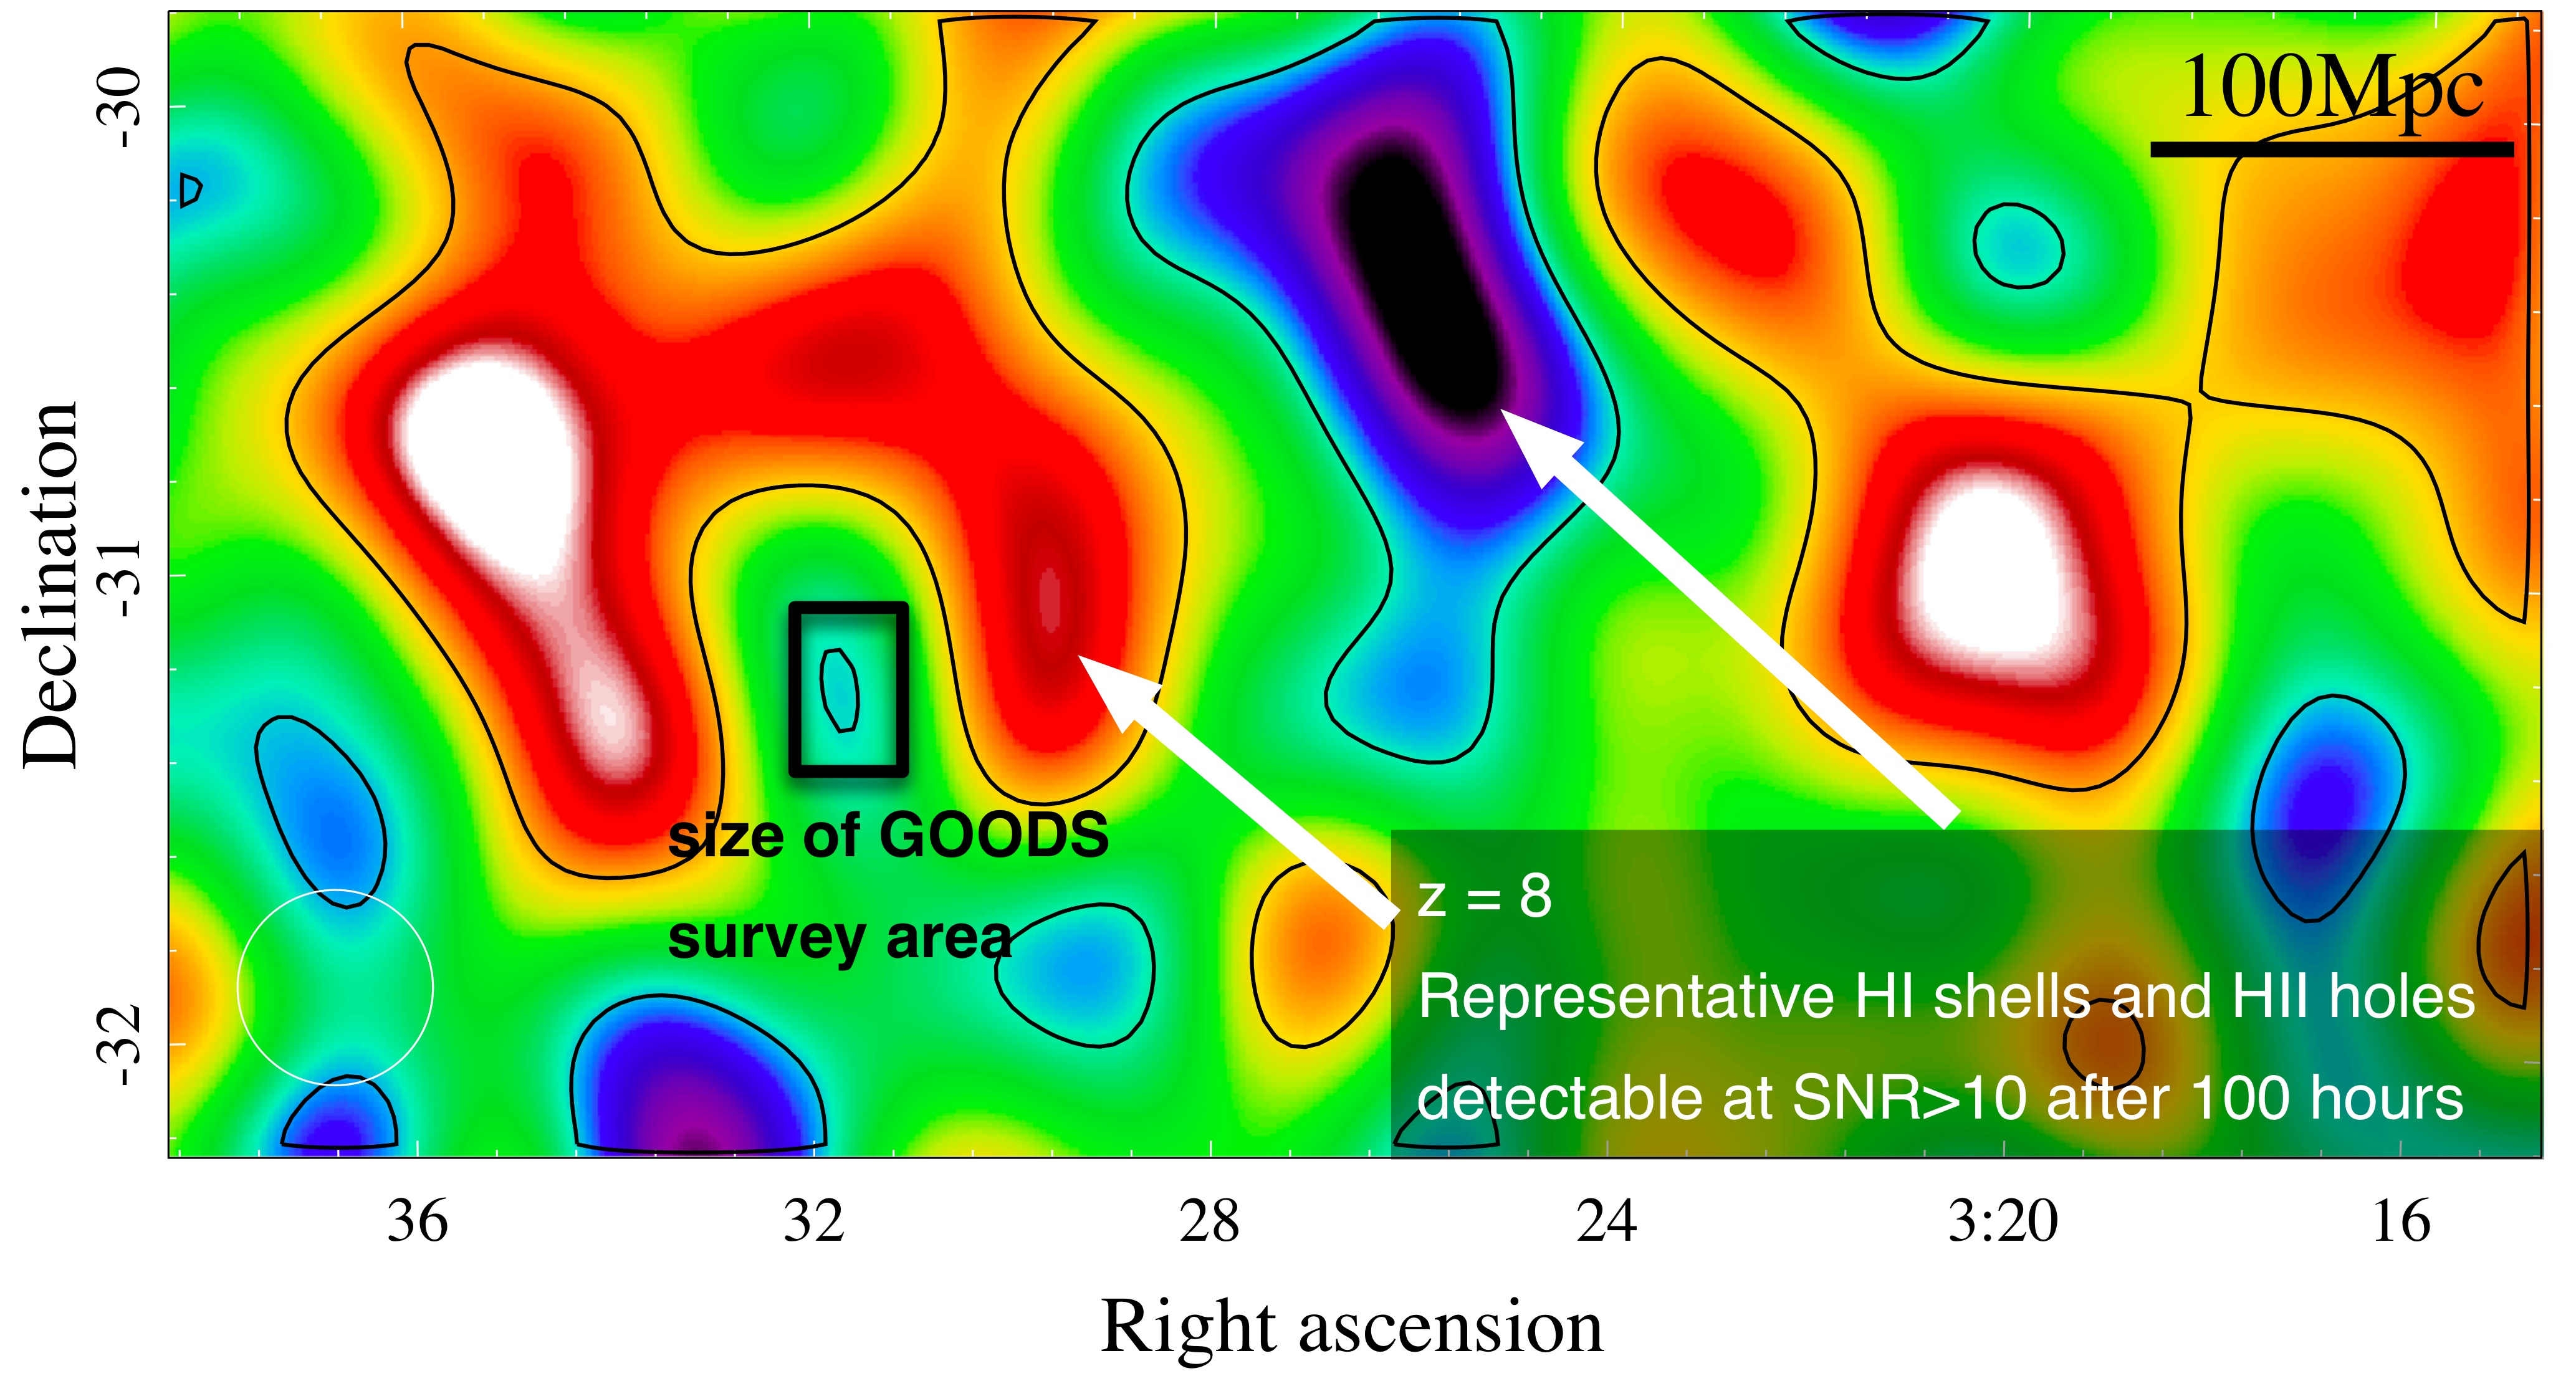
\includegraphics[height=2.5in]{HERA_331_z8_SNR_annotated.jpg}
%\caption{\small
%With sensitivity highly concentrated at the largest scales, 
%HERA-331 will have the sensitivity to directly image HI during reionization.  Shown here is a simulation of EoR emission \citep{mcquinn_et_al2007} as imaged by HERA in 100 hours of observation.  
%Contours enclose regions with signal to noise above 10.  
%With a nearly completely sampled aperture over 300~m across, HERA will have the collecting area of Arecibo but with $500\times$ the survey speed. Each night, HERA drift scans 2600 square degrees.
%}  \label{fig:imaging}
%\end{figure}    

The ability of HERA to image enables an exciting range of cross-correlation science.
HERA HI images reveal the large-scale reionization environment for pointed ALMA and
JWST observations, and other deep near-IR surveys \citep{lidz_et_al2009}. Knowing
whether an observed galaxy is in a region that was previously reionized (center of
large HII bubble), recently reionized (edge of HII bubble), or is forming from
pristine neutral gas provides important contextual information on early galaxy
formation.

The HI images can be cross-correlated with other diffuse tracers of large scale
structure. A number of studies have proposed cross-correlation with large scale
intensity mapping of molecular CO \cite{lidz_et_al2011} and atomic CII
\citep{gong_et_al2011} lines. These studies trace the large scale galaxy distribution
-- the sources of reionization. Prototypes of these experiments may be operating on
the HERA timescale. Such probes have the advantage of having different systematics
compared to HERA, potentially allowing clean measurements of the underlying signal.


VERY SHORT DISCUSSION OF WHAT LIMITS THE EOR BETWEEN Z~12-~6

\section{Background}
\label{sec:background}
\subsection{Hubble's Law}
\label{sec:hubble}
Modern cosmology has provided a spectacular understanding of the cosmic history of
our Universe starting from the instantaneous moment after the explosion of our
spacetime that we call ``the Big Bang'', which occurred about 13.8 Gyr ago, to the
advent of the large structures that seeded our cosmic current structure. After the
Big Bang, matter and space went streaming outward and is manifest to us by the simple
expression called Hubble's Law:
\begin{equation}
v = H_od
\end{equation}
where $v$ is the velocity of the object away from us, $d$ is the distance to the
object $H_o$ is the so-called ``Hubble Constant'', which has a value of 68 Mpc/km/sec
\ref{planck}, in astronomer's units, where Mpc denotes megaparsecs, where a parsec is
$3.086 \times 10^13$ km. Using measured Doppler shifts one may determine $v$, so if one
knows $H_o$ one may directly compute the distance to the object. Velocity is
typically given as a ``redshift'', denoted as $z$, related to one another by the
non-relativistic Doppler shift equation $z \sim v/c$, where $c$ is the speed of light
in vacuo. And then by Hubble's Law, that redshift conveys a distance.

Note that Hubble's ``Constant'' is a function of time and using $H_o$ denotes today's
value. Determining the evolution of Hubble's constant is essentially the role of
cosmological studies and using Hubble's law for very distant sources requires an
integration with cosmological evolution encoded within it. The values here are
derived from \ref{ned_evo}.

\subsection{Power Spectrum}
\label{sec:pspec}
One tool that is typically employed in studying large scale parameters of the
Universe, is to collapse the richness of its spatial variation to its spatial Fourier
transform and compute a power spectrum of this. It is the parameters of this power
spectrum that may be predicted by cosmology, rather than the essentially random
particular spatial variation about it. It is analogous to the fact that one may get a few broad
parameters of an FM signal by Fourier transforming its time series, regardless of whether it is
Beethoven or M\"{o}tley Cr\"{u}e, which have very different values as a function of time.

Cosmology typically encodes this data as power in spherical harmonics.  Epoch of
Reionization studies typically use wavevectors, $\k$.  This 3-D vector may be decomposed
into plane-of-sky values (${\bf \kperp}$) and a line-of-sight term (${\kpar}$).  The overall
wavevector may then be written as $\k = {\bf \kperp} + \kpar{\bf z}$.  As a wavevector,
the units of $\k$ are 1/Mpc (inverse length).  Note that although modern cosmology believes
it has pegged the value of Hubble's constant, to hedge their bets, they will often factor out
$h=H_o/100$ as an overall scale adjustment, such that the wavevector ``units'' are $h$/Mpc.  The units
of the power spectrum magnitudes are given in $\k$-volume-adjusted power-squared (mK$^2$), denoted
$\Delta ^2$.

Note that the initial approach to detecting and characterizing the EOR is therefore not imaging, but 
to detect power in a few of the power spectrum bins.  One 
may exploit this to get more samples of the power in specific bins to beat down the noise, at the expense of 
imaging, although for very compact arrays there is less of an imaging penalty as more of the bins
are filled within a radius of support.  The implications of the configuration to the array sensitivity
will be touched upon below.

\subsection{Foregrounds and Overall Signal Levels}
\label{sec:foregrounds}
At the frequencies of interest (50-250 MHz), the sky as seen by a radio telescope is dominated 
by the synchrotron emission from free electrons spiralling around the magnetic fields that thread
through our Galaxy.  The magnitude of this signal varies as a power law of the frequency, as well
as position on the sky (hottest in the plane of the galaxy, cooler at the poles).  The variation spans
from about 10,000K to about 100K in equivalent temperature.  There are a few localized sources
in the sky that are even hotter to the eyes of a radio telescope.

As will be shown shortly, the signals of interest have equivalent temperatures of $<$ 10 mK, 7 to 9 
orders of magnitude below the foreground signal strengths.  The challenge is to peer through these
strong foreground signals to see the weak signal of interest below.

As stated above, the strong foreground signals may be accurately described as smooth power laws in 
frequency - a factor that may be exploited to extract the signals of interest, which have a structure
that varies fairly rapidly with frequency.

It is also interesting to note that another ``foreground'' from our perspective is the Cosmic Microwave Background.  
In this case, the detectable signal is the difference in flux between the hydrogren and the CMB.  It acts a bit like the
weatherman's "green screen", where anything in a specfic shade of green is invisible.

\subsection{Filtering}
The wedge etc

\section{Specifications}
\label{sec:spec}
The epoch of interest, the spatial scales of interest, the required sensitivity and
the frequency smoothness provide the scientific specifications needed for the array.
Details of the technique, cost, and observing strategies also provide specifications.
This section will discuss these high-level specifications.

\subsection{Frequency Range}
The rest frequency ($\nu_o$) of the hyperfine transition of neutral hydrogen is at
1420.4 MHz. This frequency gets red-shifted to lower frequencies in deep astronomical
observations due to the expansion of the Universe, as discussed above. This is
characterized by the red-shift parameter $z$ as
\begin{equation}
\centering
\label{eq:redshift}
\nu_s(z) = \nu_o/(1+z)
\end{equation}
The age of the Universe at a particular redshift is given by the cosmological model
and a key goal of cosmology is to determine those parameters, however existing models
allow us to determine these values to our desired accuracy. Figure
\ref{fig:theUniverse} plots the red-shifted frequency as a function of red-shift (the
blue curve), with the upper axis showing the cosmic evolution time since the Big Bang
(using parameters from REF PLANCK). The bandwidth for HERA is demarcated by the
horizontal dashed lines. The black dashed lines denote the ``EOR'' core bandwidth,
and the extension to the blue dotted lines is to capture earlier epochs (going lower
in frequency) and find the post-EOR ``null'' (going higher in frequency) as discussed
below. Figure \ref{fig:theUniverse} shows the mapping.


\subsection{Bandwidth Field-of-View, and Spatial Scale}
As we've seen above, the frequency at which the hydrogen transition is observed
determines the source's cosmological distance. Therefore the bandwidth of the
observations defines a linear extent along the line-of-sight in space, specified by
the frequencies at the end points. As before, one may compute this extent as a
function of redshift using a cosmological calculator. Note that at large cosmological
distances, relatively narrow bandwidths can imply very large extents, which may have
significant cosmological evolution and hence are effectively different samples of the
Universe. For HERA, this bandwidth limit is about 10 MHz or less. The cosmological
extent for 10 MHz is shown in Figure \ref{fig:heraXY}.

Telescopes have a field-of-view of the observed sky, which gives the two orthogonal
directions to the line-of-sight. A given diameter and redshift will then have a
plane-of-sky extent that with the bandwidth will define a cosmological volume. This
plane-of-sky extent for a 14-meter dish is also shown in \ref{fig:heraXY}.

\subsection{Delay and Systematics}
To exploit the smooth spectral response filtering of the foregrounds


\subsection{Sensitivity}
The sensitivity specification is to maximize performance per cost, which determines the element 
diameter ($D$) and the number of elements ($N$) subject to the constraints above.  One therefore 
needs a model of cost and performance as a function of $D$ and $N$.  Given a fairly mature element
and system design, a bottoms-up costing appropriate for element diameters from about 6-m to 20-m 
has been done for hex-numbers corresponding to element counts from 37 to 631.  The costs here
are only those associated with delivering the array to that scope on-site, so excluding development and
science.

The equation for sensitivity has been described in previous works [REFS] and depends on many parameters
related to the instrumentation, the configuration, the location, the observing strategy, etc.  A useful form for 
the proposed compact configuration is Eq 25 in Parsons et al 2012 and reproduced here:
\begin{equation}
\centering
\label{eq:sensitivity}
\begin{split}
\Delta^2_N(k) \approx 60 \left[\frac{k}{0.1h\text{Mpc}^{-1}}\right]^\frac{5}{2}
                                         \left[\frac{6 \text{MHz}}{B}\right]^\frac{1}{2}
                                         \left[\frac{1}{\Delta\ln k}\right]^\frac{1}{2} \\
                        \times       \left[\frac{\Omega}{0.76\text{sr}}\right]
                                         \left[\frac{T_\text{sys}}{500 \text{K}}\right]^2
                                         \left[\frac{6 \text{hrs}}{t_\text{per\_day}}\right]^\frac{1}{2} \\
                        \times       \left[\frac{120\text{days}}{t}\right]
                                         \left[\frac{32}{N}\right]
                                         \left[\frac{\text{10}^4f_o}{f}\right]  \text{mK}^2
\end{split}
\end{equation}
where $k$ is the magnitude of the $k$-mode, $B$ is the bandwidth, $\Delta\ln k$ is the log
of the binsize, $\Omega$ is the field-of-view, $T_{\text{sys}}$ is the system temperature, 
${t_\text{per\_day}}$ is the number of hours observed per day, $t$ is the number of days
observed, $N$ is the number of antennas, and $f_o/f$ is the configuration metric for a 
redundant array as defined in Parsons et al.

Note that $\Delta^2_N(k)$ is the standard radiometric sensitivity equation, scaled by
the volume in $k$-space, normalized by the power spectrum Fourier coefficient, and
reduced by the number of independent samples in a given $k$-mode bin, which may have
both coherent and incoherent application.

Pulling out terms relating to diameter and number, we can write Eq. \ref{eq:sensitivity} as
\begin{equation}
\label{eq:reducedSensitivity}
\Delta^2_N(k) \propto \frac{\Omega (f_o/f)}{N\sqrt{t_\text{per\_day}}} \propto \frac{(1/D^2)(1/\sqrt{N})}{N\sqrt{D}}
= D^{-\frac{5}{2}}N^{-\frac{3}{2}}
\end{equation}
where the dependencies on diameter and number have been subsituted in, noting that the expressions for $f_o/f$ and 
$t_\text{per\_day}$were derived in Parsons et al where the baselines for the close-packed array are multiples of the diameter.

For a fixed sensitivity, we may then parameterize the performance/cost ratio by the diameter.  Figure \ref{fig:costing}

\section{System Overview}
\label{sec:design}

We have achieved a
pivotal new understanding of how instrumental characteristics give rise to the
wedge of emission shown in Figure \ref{fig:twoFGViews}.  Furthermore, we have
measurements that prove the efficacy, to the sensitivity limits of current
instruments, of projecting out foreground-dominated wavemodes within the
wedge.  The HI cosmology community is now in a position to define
the top-level instrument requirements that ensure foregrounds remain bounded
within the wedge, and to specify the sensitivity needed to obtain
high-significance detections of the 21~cm reionization power spectrum under the
conservative assumption that all foreground-dominated wavemodes within the
wedge must be projected out of our measurements.
As summarized in Table \ref{tab:signif} (see \citealt{pober_et_al2014} for more details),
based on these assumptions, current instruments are likely to achieve,
at best, only marginal detections of power from reionization.

%HERA follows the vision delineated in NWNH where the MWA and PAPER
%characterized the foreground emission and performed the first deep
%integrations, followed by a more powerful instrument that drew on the lessons
%learned and merged the scientific teams. The MWA, PAPER, and LOFAR have all
%recently started deep integrations with hopes of detecting the 21~cm
%signal.
%However, as summarized in Table \ref{tab:signif} (see \citealt{pober_et_al2014} for more details),
%these instruments are likely to achieve
%at best only marginal detections of power from reionization.
%While this might qualify as a ``detection'' if the signal is strong, the
%\emph{science} of reionization observations is beyond their reach. 
%However, the profound contributions of MWA and PAPER should not be overlooked. PAPER and the MWA have succeeded magnificently in characterizing the foreground emission, discovering the EoR window, and understanding how to remove foreground contamination from the measurements. Further, they have developed and retired the risk associated with all of HERA's major systems. 
%HERA uses these lessons perform the science of reionization, at a much lower cost than assumed in NWNH.
%% that this proposal is cheaper than NWNH suggested but never give either that
%% number nor your estimated cost.

This proposal targets two arrays: a 127-element array that borrows heavily
from components of the PAPER experiment, and an upgraded 331-element array that
incorporates several performance optimizations.  
These arrays are developed over four years (see Fig. \ref{fig:timeline} and the Project Management Plan for details),
with recurring cycles of development, testing, review, deployment, commissioning, and observation.
As listed in Table \ref{tab:signif}, the specifications of HERA-127
and HERA-331 have been set to meet precisely the requirements for obtaining,
respectively, a 10$\sigma$ detection of the 21~cm reionization signal across a broad range of redshifts, and a
25$\sigma$ detection of the power spectrum of fluctuations in the 21~cm signal
capable of determining the nature and distribution of the first galaxies that
dominate cosmic reionization.  
As discussed in
\S\ref{sec:Lessons}, these science requirements translate directly into
requirements for signal delay and collecting area that, when 
combined with a cost minimization requirement, tightly
bound the HERA design.  The basic parameters are given in Table \ref{tab:BasicParameters}.

%incorporates
%our proven foreground avoidance techniques while improving
%dramatically the sensitivity relative to current experiments.  With a
%new understanding of how antenna size and separation affect
%sensitivity and foreground isolation, it has become evident a revision
%of the PAPER antenna design can yield up to 20 times the sensitivity
%per element without substantially degrading foreground isolation.
%Where PAPER's elements lack collecting area and are smaller than
%strictly required for foreground isolation, and the majority of MWA
%and LOFAR elements are spaced too widely to avoid foregrounds,
%HERA-331 employs an extremely compact array of 14-m parabolic dishes
%with PAPER-style dipole feeds (see Figure \ref{fig:hera_dish}).  The dishes
%are placed in a compact hexagonal configuration of 331 dishes supplemented by 18 outrigger dishes to achieve dense and
%highly-redundant $uv$-sampling (see Figures \ref{fig:uv_coverage} and \ref{fig:config_optics}).  The dishes have a short (4.5m) focal height to limit the
%path length of reflections, whose time-delay gives rise to chromatic
%instrumental systematics.
%
%
%% AAARRGGHH!
%%\begin{figure}[t]
%%\centering
%%	\begin{subfigure}[b]{0.46\textwidth}
%%		\includegraphics[width=\textwidth]{plots/paper_element.jpg}
%%		\caption{-0.2in}{0.99}{-0.2in}{The PAPER element (provides a clean instrumental response as a function
%%		of frequency \citep{parsons_et_al2010,parsons_et_al2012b}, which is crucial to
%%		the foreground isolation shown in Figure \ref{fig:eor_pspec}.}
%%	\end{subfigure}
%%	\quad
%%	\begin{subfigure}[b]{0.46\textwidth}
%%		\includegraphics[height=1.75in]{plots/hera_dish.png}
%%		\caption{-0.2in}{0.99}{-0.2in}{A 14m dish designed around the feed dramatically improves sensitivity while
%%		constraining the path length and amplitude of reflections to ensure that foreground 
%%		isolation is not substantially degraded.}
%%	\end{subfigure}
%%\caption{-0.2in}{0.99}{-0.2in}{PAPER and HERA elements}
%%\label{fig:hera_dish}
%%\end{figure}
%
%The size of HERA-331 dishes optimizes cost for a fixed sensitivity and
%level of foreground isolation.  The associated reduction in the number
%of antenna elements to achieve a given collecting area, combined with
%the fact that these dishes have no moving parts, are built from
%inexpensive materials, and follow a simple construction that can be
%contracted locally, makes the cost of building HERA-331 substantially
%cheaper than was anticipated in the roadmap submitted to \nwnh\ for this
%stage of the program.   
%
%HERA leverages the technical heritage of PAPER, MWA and of CASPER\footnote{Collaboration for Astronomical
%Signal Processing and Electronics Research, a Berkeley-initiated worldwide open source community that is
%developing boards, firmware and software for the astronomical community} and incorporates a
%phased implementation to mitigate against risk.  The system, technology and phased approach is discussed below
%in more detail.
%The HERA instrument design is very straightforward.  The element
%itself is a fixed zenith-pointing 14-meter segmented prime-focus paraboloid with a high screen
%to minimize cross-talk between elements (which are spaced 14.3 meters on a
%hexagonal grid).   The $f/D$ of
%the paraboloid is 0.32, so that the focal length, $f$, is less than 5 meters to meet the 
%standing wave specification at the delays of interest of more than 60 dB of attenuation at delays 
%greater than 50 ns.
%
%
%The active feed sends back the entire dual-polarization analog bandwidth on standard
%coaxial cable to an aggregation point called a ``node'', which services 
%about 15 antennas.  This cable length is kept short (35-m) to keep any standing
%wave contamination outside of the delay-space of interest for power spectrum
%measurements.  The node amplifies, filters, digitizes and transmits the signal data stream
%back to the central processing location (the Karoo Array Processing Building - KAPB).
%Figure \ref{fig:blockDiagram} shows a block diagram of the system.


As shown in Figure \ref{fig:systemOverview}, the HERA instrument has a straightforward signal
path from antenna elements
with active feeds, to nodes that digitize and aggregate signals onto an optical network,
and on to a processing building where signals are correlated and data are stored, compressed,
and shipped to a computing cluster located at U. Pennsylvania (UPenn). 

\subsection{Antenna Element}

The novel design of HERA's antenna element
(Fig. \ref{fig:hera_dish}, right panel) represents a critical advance
that enables HERA to achieve its science goals.  This 14-m
fixed zenith-pointing parabolic dish yields more than 10 times the
sensitivity of an MWA tile (and more than 20 times
that of a PAPER element), but does so without substantially degrading
our ability to isolate and remove foreground emission on the basis of
spectral smoothness.  As described above, this is done by limiting
the timescale of signal delays and reflections to under 120 ns.

Since the time it takes radio emission to propagate between adjacent antennas 
represents a significant portion of this time budget, HERA elements must be placed close together.
Recent work characterizing foregrounds suggests that 
antenna separations of $8\lambda \approx 15$m are
well-behaved to current limits \citep{pober_et_al2013,parsons_et_al2013}. This influences our
choice of a 14-m dish diameter,
which incurs 42 ns of signal delay between adjacent antennas.
The focal height (4.5 m) derives from the illumination pattern of the prime-focus
feed and the fact that reflections
between the feed and the element
%caused by imperfect impedance matching between the feed electronics and free space, 
can introduce additional signal delay. 
%With a splash cone underneath the feed to scatter reflections, we assume -20 dB
%attenuation per reflection, so that after three traversals (13.5 m; 41 ns), reflections from
%foreground emission are below the expected level of the 21~cm reionization signal.
Additional measures, such as a splash cone underneath the feed, screens that isolate feeds from one another, and 
non-metallic cabling and poles for supporting the feeds, are all aimed at minimizing
the potential for additional sources of signal reflections.
The total signal delay associated with the HERA dish design is estimated at 83 ns, leaving
headroom for reflections arising in the analog signal path.

Cost is another design constraint, including the price of construction
materials, assembly in a remote area, and maintenance over the operational
lifetime of the array.  Care has been taken to select robust and inexpensive
construction materials (PVC, concrete, utility poles, 0.25" wire cloth) and an assembly methodology that delivers the required positional
accuracy of 10 cm and surface accuracy of 2 cm given standard expertise in construction
practices for the subcontracted teams that set the poles and construct the
elements in the field.  
%JCP: "required positional accuracy" -- what drives the requirement?
Given the sensitivity and signal delay requirements, the size of HERA
dishes optimizes a global costing curve that includes the costs of the elements,
the signal path, correlation, data storage, and processing.

% ARP: removing this figure, since it appears in project management plan
%\begin{figure}[h]
%	\centering
%		\includegraphics[width=0.46\textwidth]{plots/heracles.png}
%		\includegraphics[width=0.46\textwidth]{plots/Engineering/heraclesNA.png}
%	\caption{\small
%		The construction prototype element in California (left) with preliminary 
%        reflection measurements (right).
%} \label{fig:heracles}
%\end{figure}

%As illustrated in Figure \ref{fig:heracles}, 
A first prototype of the HERA dish is nearly completely constructed.  In this
proposal, UC Berkeley and NRAO 
lead the incorporation of lessons from the
construction process and reflectometry tests into the design.
Two further prototype elements are constructed in the first year alongside the existing
PAPER array in Green Bank, WV,
for on-sky measurements of the beam pattern and spectral 
response.
These measurements are coupled with full electromagnetic modeling to test
and refine the element design prior to a Critical Design Review at the end of the first project
year.  Three revised elements are then constructed in South Africa, involving
lead members of the construction subcontract teams for a Project Readiness Review.  %Thereafter,
%element construction will proceed continously through the second and third project years during the day,
%with a staged incorporation of new elements for night-time observing.

%The elements are
%also nearly abutting one another, which allows for sharing of physical support
%infrastructure.


% ARP: lack room for this figure.
%\begin{figure}[h]
%	\centering
%	\begin{subfigure}[b]{0.46\textwidth}
%		\includegraphics[width=0.99\textwidth]{plots/Engineering/nvsd.png}
%		\caption{Costing model for a fixed sensitivity and varying the diameter.   The arrows indicate the regions of 
%				increasing systematics and delay-space contamination.}
%		\label{fig:nvsd} 
%	\end{subfigure}
%	\quad
%	\begin{subfigure}[b]{0.46\textwidth}
%		\includegraphics[width=0.8\textwidth]{plots/Engineering/focalEff.png}
%		\caption{Analytical model efficiency of a parabolic element as a function of focal height and diameter.   The delay 
%				contamination specification is $f<5$m.}
%		\label{fig:disheffic}
%	\end{subfigure}
%	\caption{Cost and performance variational analysis data for the element.}
%\end{figure}

% FOLLOWING SEEMS TOO DETAILED FOR A PROPOSAL
%To distinguish between measured sky delays and instrumental-induced delays at a required threshold ($R_T$) dB, 
%we need sufficient attenuation of the reflected signals at a given focal length ($f$) at a specified delay ($\tau_{d}$).  Assuming a conservative simple model that the magnitude of the reflection is attenuated by $A$ dB at each reflection 
%we see that for a delay length limit of $\delta_{d}=c\tau_{d}$ and focal length $f$,  the required focal length is
%
%\begin{equation}
%f < \left(\frac{A}{R_T}\right)\delta_d.
%\end{equation}
%
%Using nominal values of $R_T$ =  60dB (an order of
%magnitude below where EoR is predicted to be below foregrounds) at delays
%corresponding to the time it takes travel 15m and a net attenuation of 20 dB per reflection, 
%we find that the focal length should be less than about 5 m.  Free-space loss effects would 
%increase that value, loosening the constraint.
%DETAILEND

%In addition to the constraints given by the element itself, the HERA element size is
%also influenced by the location of the ``knee'' in the EoR power spectrum \citep{lidz_et_al2008}
%The EoR power spectrum has an upward slope for low $k$-modes which levels off
%around $k=0.15 h$/Mpc %(see fig blah). 
%Working inside this $k$-mode would be beneficial due to the fact foregrounds are
%less problematic. This poses a problem because without knowing the
%width of our foregrounds, we can't say for sure which $k$-modes (in the power
%spectrum) are corrupted. This uncertainty, coupled with increasing systematic affects for shorter 
%baselines (hence smaller diameters), favors larger diameter antennas.

%% ARP: no room for this figure.
%\begin{figure}[h]
%	\centering
%	\begin{subfigure}[b]{0.46\textwidth}
%		\includegraphics[width=0.85\textwidth]{plots/dish.png}
%		\caption{CAD model of 14m dish with screening and some supports removed to show detail.}
%		\label{fig:dish} 
%	\end{subfigure}
%\quad
%	\begin{subfigure}[b]{0.46\textwidth}
%		\includegraphics[width=\textwidth]{plots/Engineering/hera_beam.png}
%		\caption{Analytical model beam patterns at 10m, 12m and 14m.}
%		\label{fig:beam} 
%	\end{subfigure}
%	\caption{HERA element and beam pattern.}
%\end{figure}

%The $k$-mode for a $14m$ baseline is $k = 0.023$, given by $k_{H} =
%\frac{B}{c}\frac{dk}{d\eta}$, where $B$ is the length of the baseline, 14m in
%our case, $c$ is the speed of light, and $\frac{dk}{d\eta}$ is the cosmological
%transfer function from delays to $k$-modes. In addition, narcissistic
%reflections add into our $k$ budget as well. The $f$ and $D$ choices above provide a $k$ budget for
%foreground widths to be within $\Delta{k}\sim{0.1}$. Testing these hypothesis
%and again, finding a compromise between maximum sensitivity, foreground budget
%will be key to testing and constructing the required element. Foreground width constraints
%are still an area of active research \citep{pober_et_al2013}.

% The core defining elements in this design are the central hub and three tall support poles.  Three intermediate 
% support posts are installed between each pair of poles.  A 2$^{\prime\prime}$ PVC spar of 24.1$^{\prime}$ 
% terminates at each pole and post.  These spars are supported at each end and one point in the middle at the 
% proper height and angle.  The intervening PVC pipe essentially acts as a smoothing filter between those 
% points, noting also that a beam with point loads attains nearly the quadratic shape desired.  The CAD model is 
% shown in the right panel of Figure \ref{fig:hera_dish}.  
% 
% The tall ($\sim$ 7m) poles provide locational accuracy (in all three dimensions) for the overall array installation.  
% Using conventional commercial pole-installation techniques the poles are installed first for the entire array.  
% Note that every pole except for the edge poles are shared by three antennas.  A standard theodolite can 
% then be used to mark a known level height on all three poles.  These locations are then used with tensioned 
% lines to define the center of that element and the hub is positioned at that location using a jig.
% 
% The hub uses concentric commercially available ``sonotube'' forms (circular cardboard forms for concrete pillars) 
% and PVC sleeves to hold the PVC spars and PVC supports.  The retaining holes may be accurately cut into 
% the forms, sleeves installed and concrete poured to make a simple hub to the desired accuracy.  The jig holds 
% the concentric rings in place and allows it to be centered by tensioned lines while the concrete is poured.  
% When the concrete cures one can then transfer an accurate offset from the dish vertex back to the poles.
% The intermediate posts are then located by the support sub-assemblies attached to the poles and posts along 
% with the rim sub-assemblies.  These are positioned and a small pier is poured to locate them.  After spar support 
% pieces are installed on the posts, the spars themselves and the metal cloth can be installed.
% 
% The feed is held off the three tall poles using tensioned lines to accurately locate it over the hub.  A precise 
% length of kevlar rope holds the feed down to the hub at a precise focal point.  The RF cables follow the line 
% down and out to the analog-to-digital converters and correlator.  
% 
% To minimize cross-talk, metal screens are strung between every pole/post, which go to the level of the feed.  
% The dishes have a rim-to-rim spacing of 30cm to allow the screen to be slightly angled to minimize standing waves.

\subsection{Array Configuration}

 Figure \ref{fig:config}

For HERA-127 and HERA-331, elements are arranged in a compact hexagonal grid.
This configuration minimizes antenna separation, which is critical for meeting
the science requirements for foreground isolation, and 
produces a highly redundant sampling of the $uv$ plane.  As described in
\S\ref{sec:Lessons}, redundant configurations have been employed by PAPER to
boost sensitivity \citep{parsons_et_al2012a}, with the added benefit that they
greatly facilitate fast and accurate calibration
\citep{liu_et_al2010,parsons_et_al2013}.  Placing HERA elements in a
grid allows certain construction components to be re-used between antennas,
reducing cost and improving the accuracy of element placement.  HERA-331 
is a build-out of HERA-127 from the eastern edge.

The HERA-331 core has excellent
imaging capability that can be leveraged for developing foreground suppression techniques
to improve access to the 21~cm reionization signal 
(Fig. \ref{fig:eor_pspec}, black).
This capability is augmented with 21 outrigger elements.  These outriggers
combine with the dense core to generate a fully
sampled $uv$ plane out to 400$\lambda$.  While outriggers on the southern half of the array are
placed in alignment with the hexagonal grid in the core, elements on the northern side are
shifted off-grid to sample the $uv$ plane at sub-aperture scales.
This sampling strategy helps eliminate grating lobes in the
synthesized beam and provides information for
calibrating and correcting direction-dependent antenna responses.  This capability may
be used to match polarization beams and minimize
polarization leakage.

\subsection{Analog Signal Path}

HERA's analog signal path inherits directly from PAPER.
In keeping with a philosophy of
incremental change,
HERA-127 reuses the tested and commissioned feed, LNA, cables, and post-amplifier gain modules
(Fig. \ref{fig:components}, left and center) that are currently being
used to good effect in PAPER-128 \citep{parsons_et_al2010}.  Existing PAPER feeds are attached to new
reflector screens that are suspended over the elements, but otherwise remain unmodified.
A parallel development effort in NRAO aims to improve the feed response below
100 MHz 
and to improve the match between polarization beams in the feed-element system.  
Additional
minor modifications to the analog signal path include transitioning from a 75$\Omega$ to a
shorter 50$\Omega$ cabling system and replacing 100--200 MHz bandpass filters with 50--250 MHz equivalents.
This wider analog bandwidth is used in HERA analysis to improve the extrapolation of smooth foreground
emission over a broader range, and to explore HERA's capability as a Dark-Ages science instrument.
After a Critical Design Review, the results of these development efforts are incorporated in
the transition to the HERA-331 system.  


\subsection{Digital System}
\label{sec:digital}

\begin{figure}[t]\centering
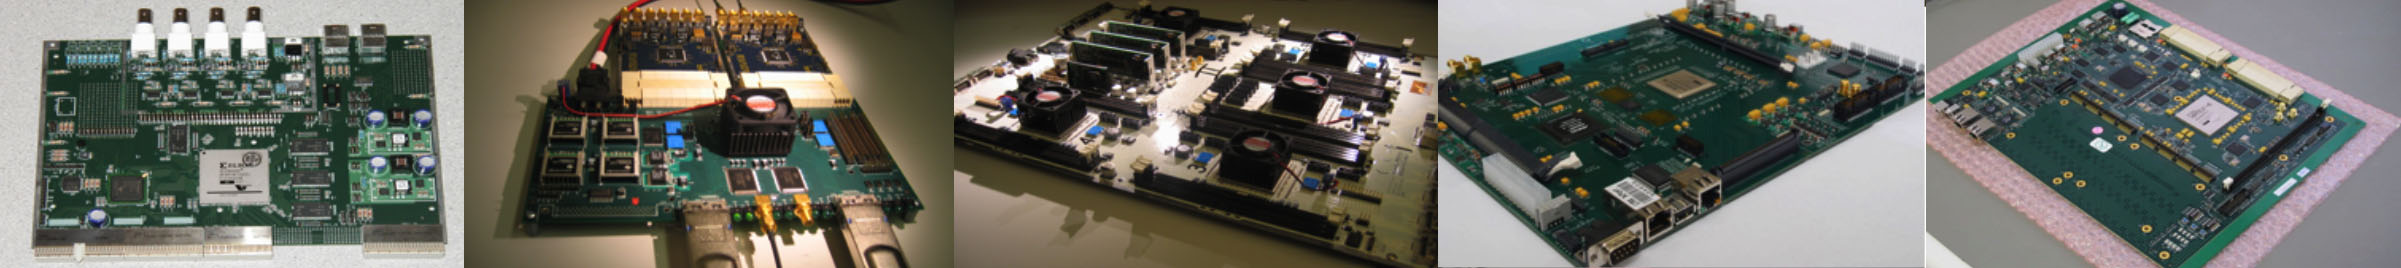
\includegraphics[width=6.5in]{plots/casper_boards.jpg}
\caption{-0.3in}{0.99}{-0.15in}{\small
Five generations of CASPER technology (progressing left to right) have been used to rapidly
develop, test, and deploy digital instrumentation for radio astronomy.  This technology
allows the PAPER correlator to be 
easily upgraded for HERA, incorporating new technology
\citep{parsons_et_al2006,parsons_et_al2008}.
}\label{fig:casper_boards}
\end{figure}

%HERA's digital system continues in the vein of PAPER's digital correlators.
Although correlators have historically been one of the most complex,
expensive, and risky aspects of developing a radio interferometer, this is no longer the case.
CASPER \citep{parsons_et_al2006}
open-sourced the development of digital signal processing engines for astronomy and
now has world-wide participation,
with over 500 members at 73 institutions, and 
five generations of hardware (Fig. \ref{fig:casper_boards}). 
On a modest budget, PAPER has applied CASPER technology to develop and deploy new correlators
annually for five years running, each quadrupling the computational capacity of its predecessor.
Led at UC Berkeley's Radio Astronomy Lab (RAL),
HERA efforts continue this incremental development cycle, following a packet-switched
correlator architecture \citep{parsons_et_al2008} that has been
extended in recent PAPER and LEDA deployments (Fig. \ref{fig:components}, right)
to leverage the computing strengths of both FPGAs and GPUs \citep{clark_et_al2011}.

While HERA-127 uses the existing PAPER correlator directly, this correlator architecture evolves for
HERA-331.  As discussed in previous sections,
HERA's science requirements dictate a maximum analog signal path-length.  As a consequence,
digitization needs to happen close to the antenna
elements in the field.  This specification, along with a growing need for modularity to scale with the number of parallel signal paths,
leads HERA to adopt a node-based architecture for amplification, digitization, channelization, and digital
transmission in the field that builds on HERA's MWA heritage.  This architecture is merged with PAPER's clean 
architecture for real-sampling and channelizing the entire analog passband at once, packetizing the data into
10 Gb Ethernet format, and relying on commercial switches to perform the frequency/antenna corner-turn that
FX correlator architectures require. 

%\begin{figure}[t]\centering
%%\includegraphics[width=6.5in]{plots/node_arch.png}
%\caption{
% something about nodes here.  Maybe also block diagram of NRAO digitizer board.
%}\label{fig:node_arch}
%\end{figure}


{\bf Node}. HERA-331 employs RFI-tight node enclosures that each contain the final gain and digitization stages for
signals from 18 antennas, along with power supplies, cooling, and a small server for monitor/control.  
As part of HERA development,
a new board called the Smart Network ADC Processor (SNAP) board is incorporated 
into the CASPER suite of hardware and firmware. This inexpensive board was co-designed by UC Berkeley and NRAO to be
both the digitizer and F-engine in HERA's FX correlator architecture,
and is currently in layout at NRAO.  Each SNAP board 
digitizes and channelizes a 50--250 MHz band for 6 input signals (3 antennas, dual-polarization).
A 100-MHz band of selectable channels is transmitted over optical fiber
to a central container (see below), and on to the Karoo Array Processing Building (KAPB).  The development and integration of the SNAP
design and the node system is led at UC Berkeley and after a Critical Design Review, is fabricated
under subcontracts to industry partners in the third project year and deployed as part of the HERA-331 system.
Development activities under this proposal include porting the CASPER toolflow to
the SNAP board, designing and testing the FPGA firmware,
integrating and testing all components in the node subsystem, and providing a monitor/control
access interface.  If time allows, optional development may include doubling the transmitted bandwidth.

{\bf Central Container}.
HERA's central container houses two significant subsystems adjacent to the array.  The first is a timing subsystem
that maintains a GPS-disciplined oscillator and distributes timing
signals (the sampling clock and 1PPS synchronization) to the nodes.  The second
subsystem is a passive fiber optic patch panel that couples
the optical network from the nodes into the 192-filament optical fiber bundle 
that connects to the KAPB. 

{\bf Karoo Array Processing Building (KAPB)}.
The KAPB is currently
in advanced stages of construction for MeerKAT, and houses the switch and processors
that 
complete the HERA correlator system.  The fiber optic bundle that enters the KAPB patches
into local fiber optic cables 
that each terminate in optical transceivers that plug into a 240-port 10 GbE switch.
Such switches, while large, are readily available commercially today.  Also connected to
this switch are 30 servers, each hosting two dual-GPU graphics cards and two dual
10 GbE network interface cards, which implement the cross-multiplication (X-Engine) component
of the correlator during observations.  This estimate for the number of X-Engine servers
is extrapolated from current GPU servers deployed on PAPER, assuming no improvement in bus
speeds for transferring data into the GPU cores, but assuming that the computational
capacity of such GPU cores doubles according to Moore's Law prior to the purchase of
these servers in the third year of the project.
Output data from the correlator are written to the data storage system described
in the following section.

%C. Post correlator data path
% Aguirre, Moore

\subsection{Data Storage, Compression, Transfer, and Computing}
\label{sec:data}

HERA's data management system is responsible for recording raw data from the
correlator, compressing that data in real-time, applying routine calibration
and analysis pipelines, and transferring data products to 
a high-performance computing cluster at UPenn.
UPenn leads the procurement
and deployment of three data storage systems:
\begin{itemize}%[noitemsep,nolistsep]
\item a 1.5 PB system deployed in the KAPB for archiving all 1.2 PB of raw data and 60 TB of compressed data, 
\item 6 network attached storage (NAS) units plus 2 125 TB RAID array units that are used to ship compressed data products to the US, and
\item a permanent 250 TB system at UPenn associated with a computing cluster that
holds compressed data products and serves as the analysis engine for HERA collaborators.
\end{itemize}
\noindent
This effort leverages existing infrastructure at UPenn, with support
for the expansion of the data storage and for upgrading to a 30-node computing cluster.  This cluster supports the bulk of the analysis by HERA collaborators (see \S\ref{sec:analysis}) that requires access to the full set of HERA observations.

%The main data center at Penn will house all of the maximally compressed data from all seasons of HERA, as well as the LST-averaged data.  The storage system is sized so that there is a factor of 4 overhead for work on the maximally-compressed data set, and a factor of 2 on the LST-averaged. The 500 TB data storage will be coupled to a 32-node cluster which performs the tasks of calibration and averaging to further reduce the data volume.  This cluster will support the bulk of the analysis requiring the full data set.  Subsets will be served off to collaborators from this system.  The entire data storage and transfer plan for HERA draws heavily on the experience with PAPER data.

The data compression scheme at the heart of the data management system
has been implemented for PAPER (\citealt{parsons_et_al2013},
Appendix A), and is applied to HERA visibilities to reduce data volume by
a factor of $\sim$20 without impacting reionization science
capabilities.  This compression technique, which is based on delay/delay-rate
filtering \citep{parsons_backer2009}, is applied uniformly to all visibilities
in the array, does not require (or produce) detailed calibration
information, and is minimally restrictive for how data are analyzed and calibrated afterward.
Data compression is run on the same GPU servers
that implement the correlator X-Engines (\S\ref{sec:digital}).  Since HERA only observes at night,
these processors would otherwise be unused.  UC Berkeley is responsible for porting
the existing data compression pipeline to target these servers.

Data quality assurance (QA) is performed in real time on an additional modest 
computing cluster in the
KAPB.  UPenn leads the deployment and support of the hardware system that
manages data transfer, applies routine calibration pipelines (see \S\ref{sec:analysis}) and quality
checks, and aggregates correlation-based metrics of array performance in real-time.  The QA system
furnishes this information into the separate monitor and control system (\S\ref{sec:monitor}).
A modest amount of data transfer is possible over the internet; PAPER's data transfer rate from the Karoo
to UPenn varies, but peaks around 40 Mbps.  The QA system drives internet data transfer, but
NAS devices and RAID storage, transferred by air-freight shipping, ensure full data transfer to UPenn.

%ii. transport to data centers
%In order to transfer maximally-compressed data over the internet in a timely manner, a network speed of around the instantaneous compressed data rate is required.  Negotiations with the IT SKASA and the South African internet provider (Tenet) have achieved transfer speeds between the PAPER site and the United States have been measured to be up to 40 Mbps, which easily
%accommodates the first two seasons of HERA observations.  In all seasons, however, portable, inexpensive, network-attached storage devices will be used to transfer data by air-freight shipping. 

%iii. data centers: access?

%The main data center at Penn will house all of the maximally compressed data from all seasons of HERA, as well as the LST-averaged data.  The storage system is sized so that there is a factor of 4 overhead for work on the maximally-compressed data set, and a factor of 2 on the LST-averaged. The 500 TB data storage will be coupled to a 32-node cluster which performs the tasks of calibration and averaging to further reduce the data volume.  This cluster will support the bulk of the analysis requiring the full data set.  Subsets will be served off to collaborators from this system.  The entire data storage and transfer plan for HERA draws heavily on the experience with PAPER data.

\subsection{Monitor and Control}
\label{sec:monitor}

The U. of Washington team leads the development of HERA's Monitor and Control (M\&C) system,
which is a straightforward port of a similar system used on the MWA \citep{tingay_et_al2013}.
This system is
responsible for tracking observing status, array startup and shutdown, and
monitoring all active HERA systems. In the process, the M\&C system builds a sizeable database of 
metadata that is crucial for verifying system functionality, identifying hardware failures, and feeding
calibration and contextual information into data analysis pipelines.  

%Top-level interface for controlling and monitoring major subsystems. 
%Collection of monitor data from nodes, switch, correlator, data compression, and data transfer subsystems.
%Incorporation of calibration data from real-time application of redundant calibration (cite section), as well as
%other calibration, imaging, and assessment subsystems.
%
%%\subsubsection{Array monitoring/maintenance: daily, weekly health monitoring}
%% de Boer
%
%In addition to Monitor and Control subsystem, which aggregates routine checks that are run automatically as
%part of the data compression and transfer pipeline, there is a need for deeper analysis
%exploring the data for more subtle defects, as well as monitoring progress toward sensitivity goals.
%We have set aside time for students at each institution, rotating among institutions, and managed at MIT,
%for performing such data exercises.
%Combine this with information from monitor database to identify hardware and subsystem failures.
%Aggregate lists of systems requiring maintenance attention, which are then handled by system owners
%in coordination with appropriate members of their teams.

\subsection{Software, Analysis, and Science}
\label{sec:analysis}

Beyond the construction and data-taking aspects of HERA, this proposal
incorporates a full data analysis effort, culminating in the publication of a
suite of science papers connecting observations to the physics of cosmic dawn.
These efforts leverage existing software pipelines, with on-going 
development driven by students and postdocs targeting specific science goals.
On the science side, HERA leverages the involvement of a team of theory collaborators,
including Furlanetto, Lidz, Loeb, McQuinn, Mesinger, Oh, Pritchard, Santos, and Sutter.

%\compress
%\subsubsection{Calibration}
%\label{sec:calibration} 

{\bf Calibration and Snapshot Imaging}. MIT leads
the development of a real-time redundancy-based calibration pipeline based on related
MITEoR and PAPER efforts.
These instantaneous calibration solutions are provided to
the Monitor and Control system to enable 
hardware misbehaviors to be quickly identified, and also support the
real-time imaging pipeline.  Absolute calibration is fixed with
a combination of self-calibration techniques and absolutely calibrated baluns developed at ASU and NRAO.
%Once data quality is assured, multi-day observations 
%binned in local sidereal time, and averaged. This intermediate
%averaging scheme will also generate an accurate visibility-based sky
%model for the instrument once calibration is applied.
Offline, detailed imaging efforts feed into developing
empirical beam models that
complement electromagnetic simulations.  UPenn develops polarization beam models
that determine whether polarization leakage can be formally retired as 
a risk and lay the foundation for imaging-based foreground suppression that
corrects any remaining leakage effects.

%\compress
%\subsubsection{Foreground Modeling and Removal}
%\label{sec:DataProducts}

{\bf Foreground Modeling}. The U. Washington team leads the adaptation
of a high dynamic-range imaging pipeline
based on the Fast Holographic Deconvolution (FHD; \citealt{sullivan_et_al2012}).
for HERA.  The full-Stokes sky maps resulting from this pipeline
are used to directly subtract foregrounds
and as data products themselves.  UPenn leads
the characterization of the polarized sky and the
distribution of rotation measures.  Data from HERA, PAPER, and the MWA are used
to update source catalogs and a Global
Sky Model \citep{deoliveira2008}. %providing reference sky models for both
%HERA and other low-frequency instruments. %The goal will be to generate a model
%suitable for direct subtraction of foregrounds. 

% XXX need more data products here

%\compress
%\subsubsection{Power spectrum and related measurements}

{\bf Power Spectra}. UC Berkeley leads early power spectrum measurements using the conservative
delay-spectrum approach used in PAPER.  %This
%visibility-based approach, when coupled with a foreground-avoidance strategy,
%is sufficient for an unambiguous early detection of the 21~cm
%power spectrum should results from current-generation experiments prove
%marginal (Fig. \ref{fig:eor_pspec} and Table \ref{tab:signif}).  
Development of
the power-spectrum pipeline will focus on incorporating
a fully covariant description of the foreground wedge
\citep{liu_tegmark2011,dillon_et_al2013a}, as well as
exploring Bayesian techniques for power spectrum estimation, building on the considerable
progress already made on Gibbs-sampling imaging for interferometers \citep{sutter_et_al2014}.
In addition to the statistical foreground mitigation techniques provided by optimal quadratic
power-spectrum estimation, U. Washington leads the application of 
foreground modeling for expanding the range of modes available for power spectrum analysis.
Techniques developed should be equally applicable
to measurements in both the reionization epoch and at higher redshifts.  MIT leads the application
of these tools for pre-reionization science.

{\bf Simulation}. To provide verification of power spectrum constraints, ASU leads the
development of an end-to-end simulator of the full HERA instrument, incorporating
foregrounds and reionization models to output visibilities.  UCLA also leads
a parametrized reionization simulation effort that, coupled with the instrument
simulator, is critical for connecting power-spectrum constraints to the estimation
of the underlying astrophysical models.

%\compress
%\subsubsection{HI Imaging}

{\bf HI Imaging}. In addition to supplying models for suppressing foregrounds,
deep imaging aims to map HI emission during reionization (see \S\ref{sec:science}).
Initially, conservative filtering of the foreground wedge is applied to data that
are imaged.  These results are compared with the residuals from imaging-based
foreground suppression to explore the limitations of 
precision foreground imaging and removal.  As imaging-based techniques mature, the resultant
maps are released for cross-correlation with other probes of reionization.

%\subsubsection{Aspirations [move to facilities section?]}
%
%i. FFT correlator
%ii. other


%\compress
%\subsection{Schedule} % 0.5 page
% De Boer


%\begin{table}[t]
%\centering
%\caption{Schedule Overview}
%\label{tab:scheduleSummary}
%\begin{tabular}{| p{1.5in} | p{1.5in} | p{1.5in} | p{1.5in} |}\hline
%\textbf{Year 1}:  FY2015   &  \textbf{Year 2}:  FY2016  &  \textbf{Year 3}:  FY2017 & \textbf{Year 4}:  FY2018 \\ \hline
%\raggedright{Infrastructure, prototyping and contract preparation.} &
%\raggedright{Hardware commissioning and deep foreground survey.} &
%\raggedright{HERA-127 observations:  detecting the rise and fall of reionization.} &
%HERA-331 observations:  measuring the evolution of the first galaxies. \\ \hline  %It won't let me make this one raggedright!
%\begin{itemize}[noitemsep,nolistsep,leftmargin=12pt]
%\item Basic infrastructure
%\item GB, SA prototypes
%\item Design package
%\item Polarization software
%\end{itemize} &
%\begin{itemize}[noitemsep,nolistsep,leftmargin=12pt]
%\item HERA beam pattern
%\item HERA-127
%\item Delay-spectrum/FHD software
%\item Analysis pipelines
%\end{itemize} &
%\begin{itemize}[noitemsep,nolistsep,leftmargin=12pt]
%\item HERA-127 observations
%\item Electronics upgrade
%\item HERA-331
%\item HERA-127 analysis
%\end{itemize} &
%\begin{itemize}[noitemsep,nolistsep,leftmargin=12pt]
%\item HERA-331 observations
%\item Cross-correlations
%\item Cosmological simulations
%\end{itemize} \\ \hline
%\end{tabular}
%\end{table}

% need to discuss in a few sentences the
% relation to other experiments in the same time frame.

%\begin{itemize}[noitemsep,nolistsep]
%\item{Year 1:} Infrastructure, Prototyping, Contract Preparation (FY 2015).      
%\begin{itemize}[noitemsep,nolistsep]
%\item Install basic infrastructure (ground leveling, power, network connectivity) for new infrastructure
%\item Incorporate existing PAPER-128 antennas, correlator, and housing container.
%\item Install additional prototypes in Green Bank and test.
%\item Define final design package for element construction
%\item Start developing improved HERA baluns, receivers, feeds, nodes, and in-situ antenna calibration system.
%\item Continue delay-spectrum, FHD, and optimal estimator software development.
%\item Develop polarization capable software for beam/leakage studies.
%\end{itemize}
%\item{Year 2:} Hardware Commissioning and Deep Foreground Survey (FY 2016).  
%\begin{itemize}[noitemsep,nolistsep]
%\item Observations using PAPER antennas in an imaging configuration.
%\item Determine on-sky beam response of HERA antennas to facilitate future source subtraction efforts.
%\item Finalize site infrastructure (high-bandwidth optical network, surveying, trenching).
%\item Commission new feeds, receivers, nodes, and calibration systems in Green Bank and SA.
%\item Complete HERA-127 construction
%\item Initial delay-spectrum, FHD, and optimal estimator software ready for HERA 127 analysis.
%\item Full end-to-end simulations of analysis pipelines.
%\end{itemize}
%\item{Year 3:} HERA 127 and Detecting the Rise and Fall of Reionization (FY 2017).  
%\begin{itemize}[noitemsep,nolistsep]
%\item HERA 127 complete. Science observations begin using the PAPER correlator.
%\item Begin deployment of HERA 331. Install new node electronics and a 331-element, GPU-based correlator in the Karoo Array Processing Building (KAPB).
%\item Install new data storage infrastructure in the KAPB.
%\item Upgrade the UPenn analysis cluster.
%\item Finish construction of HERA 331
%\item Apply proven delay-spectrum analysis techniques to HERA 127 observations to constrain the timing and duration of reionization.
%\item Multi-pipeline analysis of HERA 127 observations to compare pipeline strengths/weaknesses.
%\end{itemize}
%\item{Year 4:} HERA 331 and Measuring the Evolution of the First Galaxies (FY 2018).           
%\begin{itemize}[noitemsep,nolistsep]
%\item HERA 331 complete. Begin science observations Oct. 2017.\item Begin multi-pipeline analysis of data to characterize the evolution of the power spectrum and determining properties of the first galaxies. 
%\item Continue analysis software development: optimize existing algorithms and develop imaging-based subtraction techniques for expanding the EoR window
%\item Create high-fidelity maps/data cubes of the HERA field for cross-correlation studies
%\item Cosmological simulations for extracting reionization physics from power spectrum measurements
%\end{itemize}
%\end{itemize}

\conclusions  %% \conclusions[modified heading if necessary]
And sugar and spice


%\appendix
%\section{}    %% Appendix A
%\subsection{}                               %% Appendix A1, A2, etc.




\begin{acknowledgements}
TEXT
\end{acknowledgements}


%% REFERENCES

\bibliographystyle{copernicus}
\bibliography{biblio}
%%
%% URLs and DOIs can be entered in your BibTeX file as:
%%
%% URL = {http://www.xyz.org/~jones/idx_g.htm}
%% DOI = {10.5194/xyz}

%% LITERATURE CITATIONS
%%
%% command                        & example result
%% \citet{jones90}|               & Jones et al. (1990)
%% \citep{jones90}|               & (Jones et al., 1990)
%% \citep{jones90,jones93}|       & (Jones et al., 1990, 1993)
%% \citep[p.~32]{jones90}|        & (Jones et al., 1990, p.~32)
%% \citep[e.g.,][]{jones90}|      & (e.g., Jones et al., 1990)
%% \citep[e.g.,][p.~32]{jones90}| & (e.g., Jones et al., 1990, p.~32)
%% \citeauthor{jones90}|          & Jones et al.
%% \citeyear{jones90}|            & 1990


%% FIGURES

%% ONE-COLUMN FIGURES

%f
\begin{figure}[t]
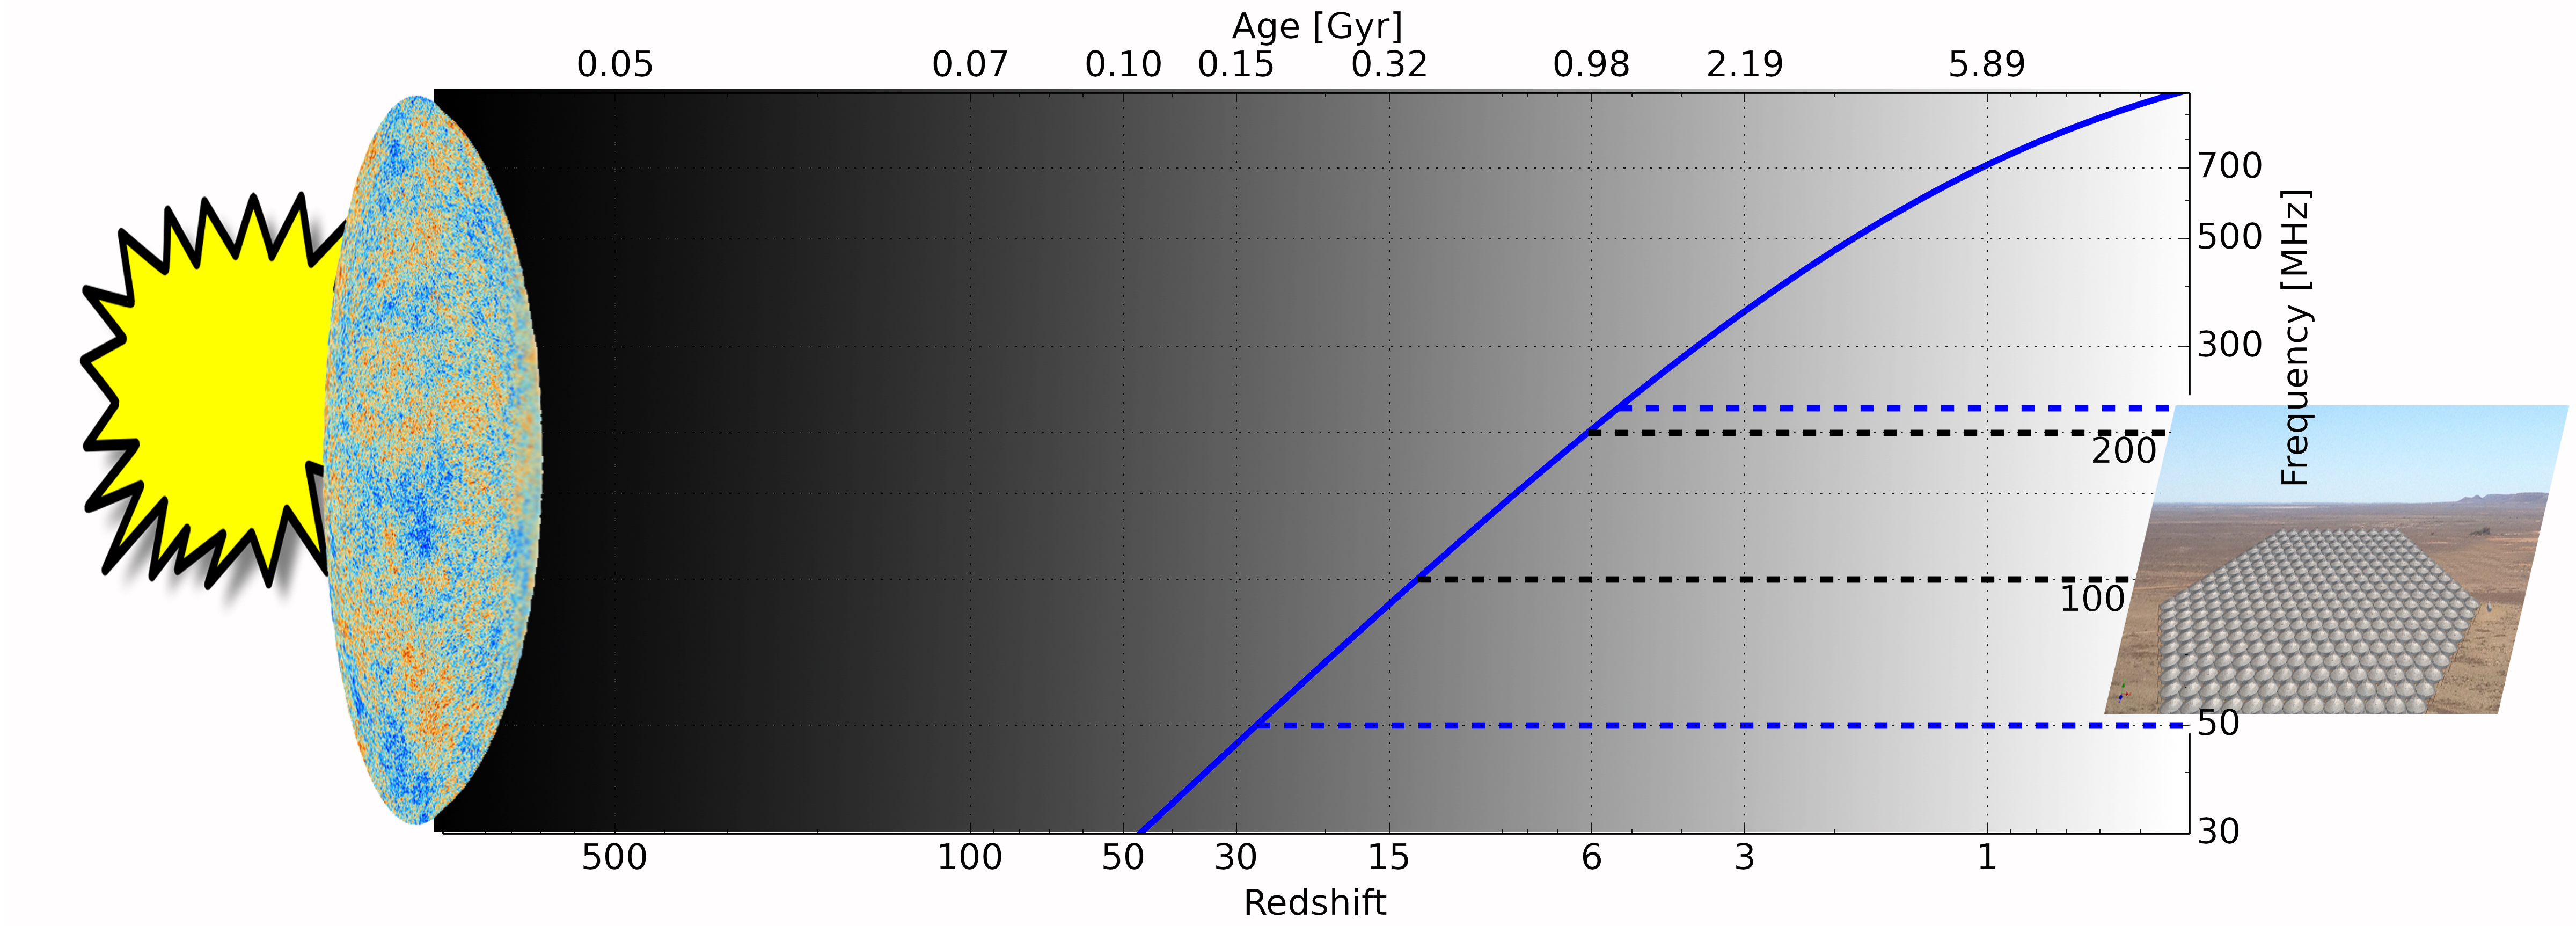
\includegraphics[width=8.3cm]{plots/herauniall.png}
\caption{\small Cartoon showing the development of the Universe and HERA's observing window into it (dashed lines).  The blue solid
line shows the \HI transition frequency as a function of redshift/cosmic evolution age.  The black dashed lines indicate the HERA EOR ``core'' band and blue dashed lines the expanded band, which are detailed in Table \ref{tab:heraband}.}
\label{fig:theUniverse}
\end{figure}

\begin{figure}[t]
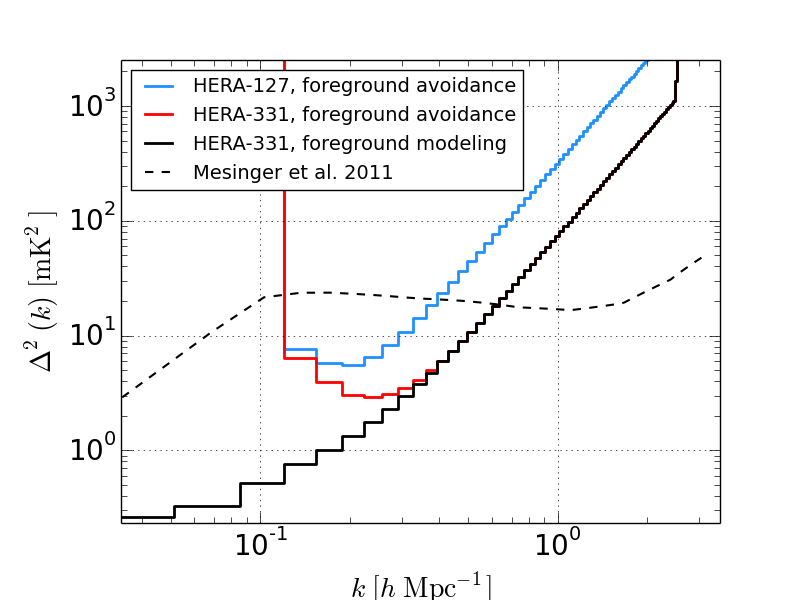
\includegraphics[width=4.1cm]{plots/eor_pspec_2014.png}
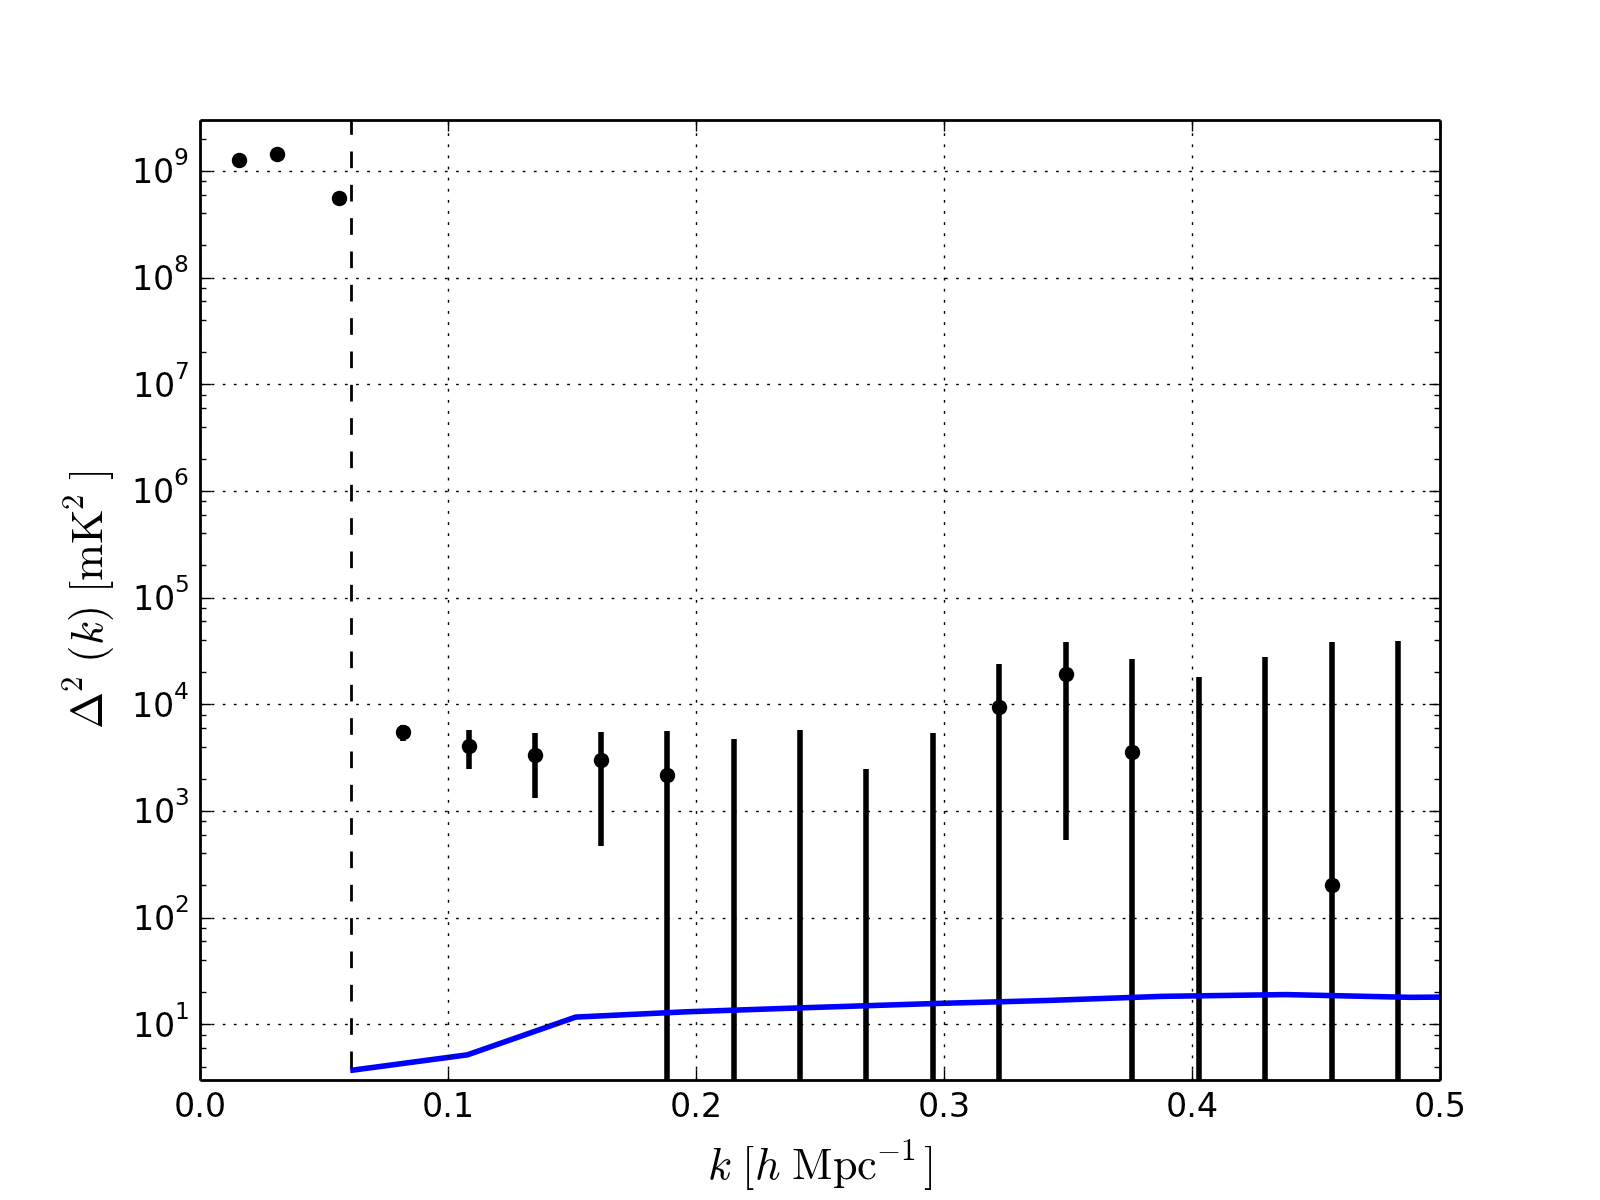
\includegraphics[width=4.1cm]{plots/hera_pk3pk.png}
\caption{\small Top: HERA's power-spectrum sensitivity (solid)
relative to a fiducial ionization model (dotted line; $\xHI=0.37$, $z=9.0$).  
Sensitivities reflect staged array size and
improving analysis software that expands the range
of modes free of foreground systematics. 
Bottom: The current best upper limit on the 21~cm reionization power spectrum,
obtained with a 32-element PAPER deployment \citep{parsons_et_al2013}.  These upper limits
constrain the brightness temperature of the IGM at $z\sim8$, showing
a departure from adiabatic cooling presumed to be indicative of X-ray heating.}
\label{fig:eor_pspec}
\end{figure}

\begin{figure}[t]
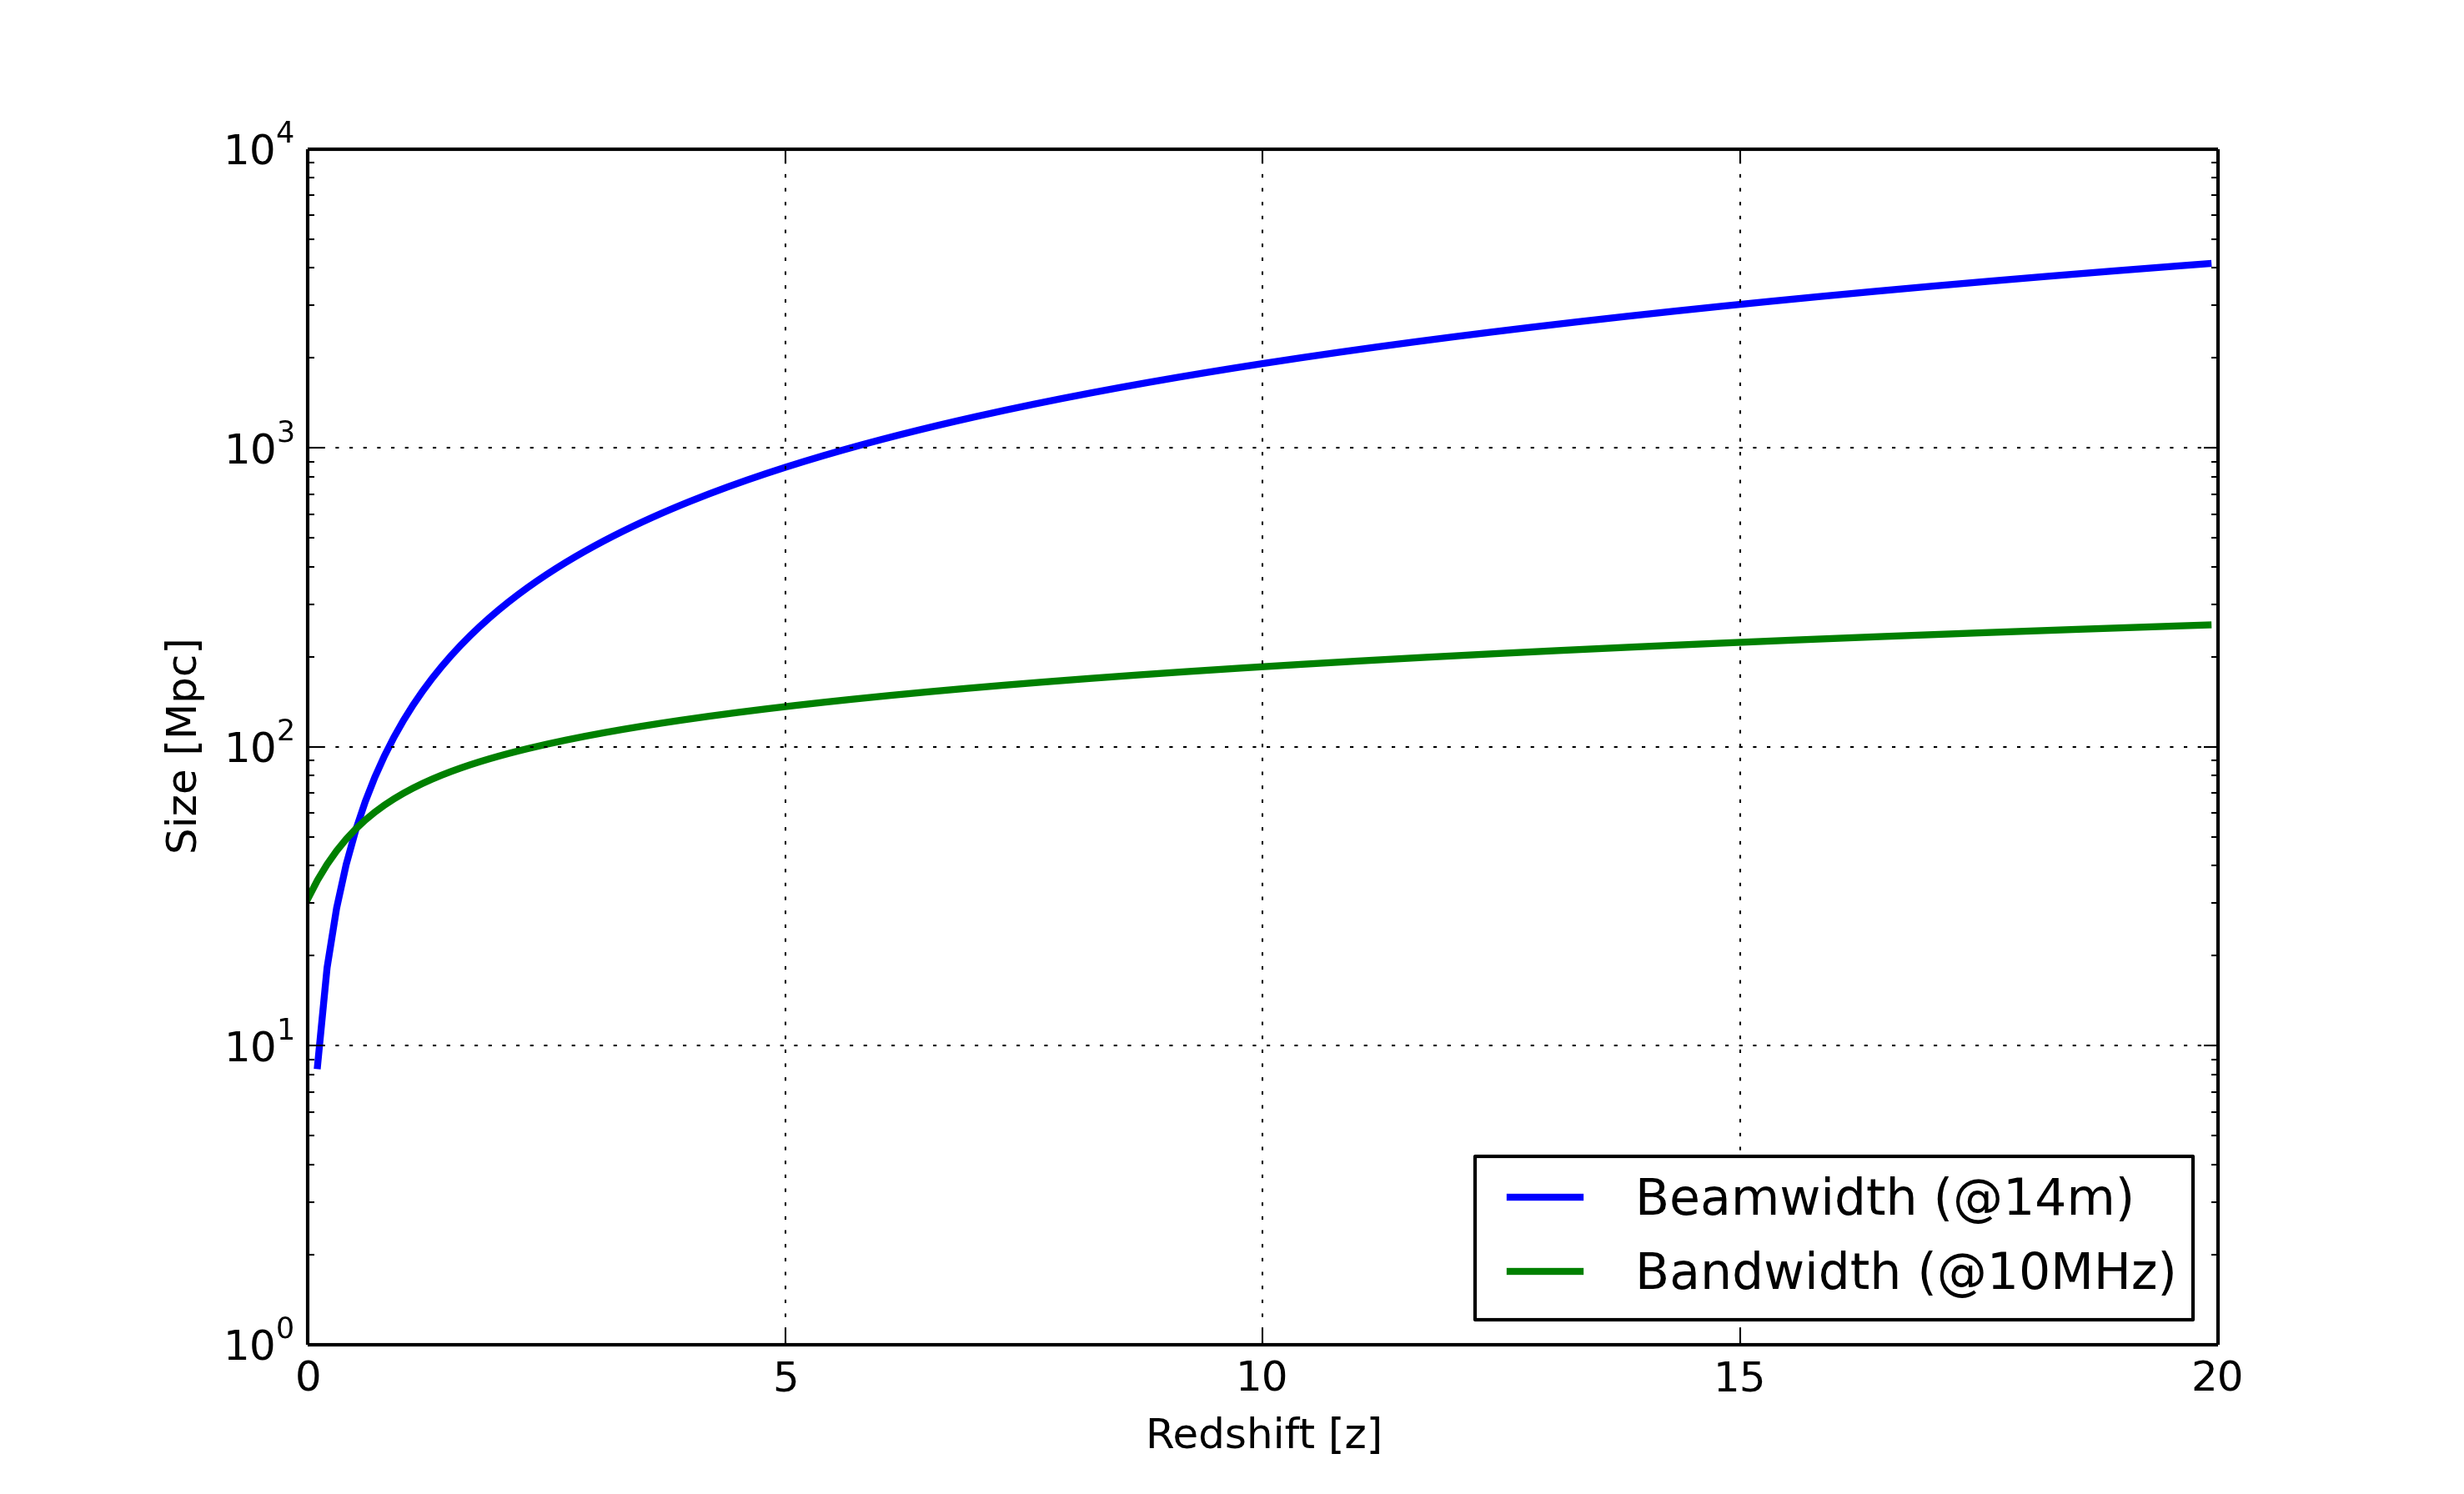
\includegraphics[width=8.3cm]{plots/heraXY.png}
\caption{\small Scaling}
\label{fig:heraXY}
\end{figure}

\begin{figure}[t]
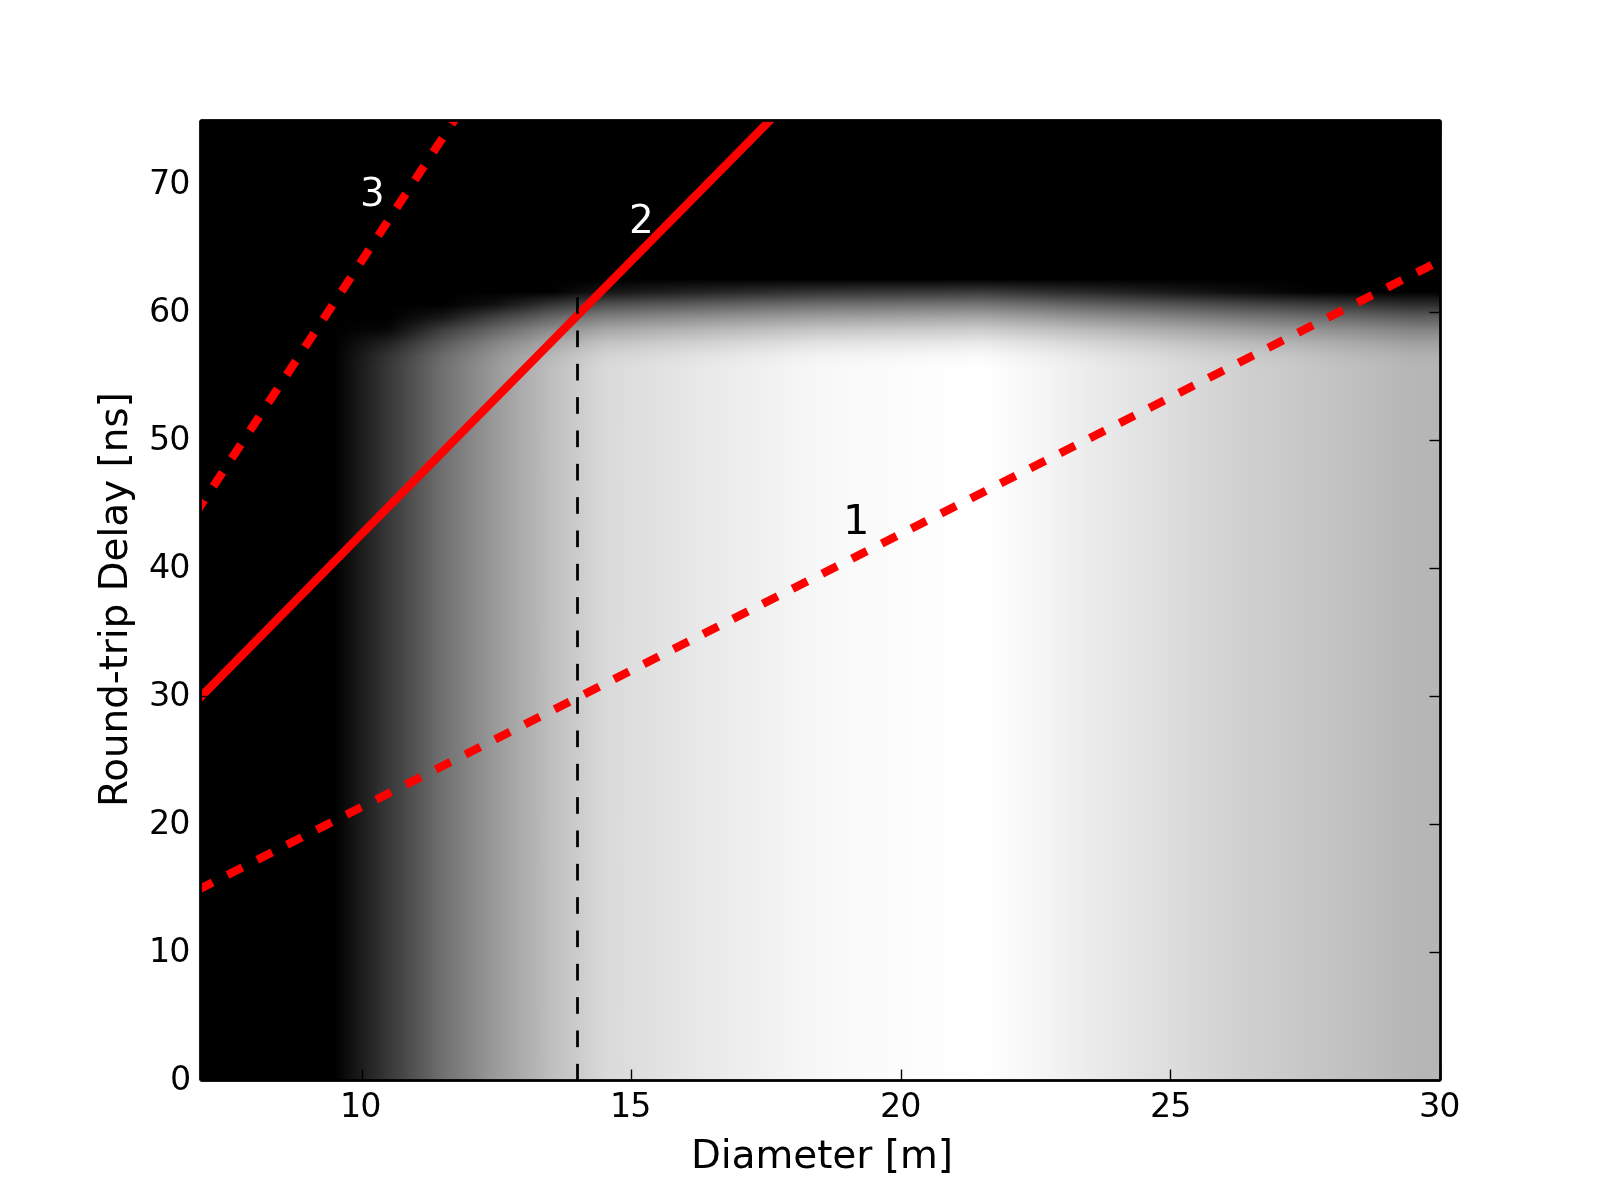
\includegraphics[width=8.3cm]{plots/costing.png}
\caption{Costing}
\label{fig:costing}
\end{figure}

\begin{figure}[t]
        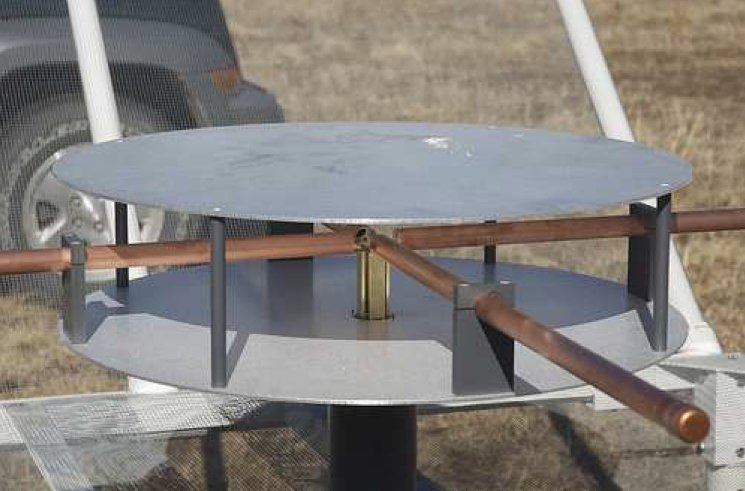
\includegraphics[width=2.7cm]{plots/new_antenna_closeup.jpg}
        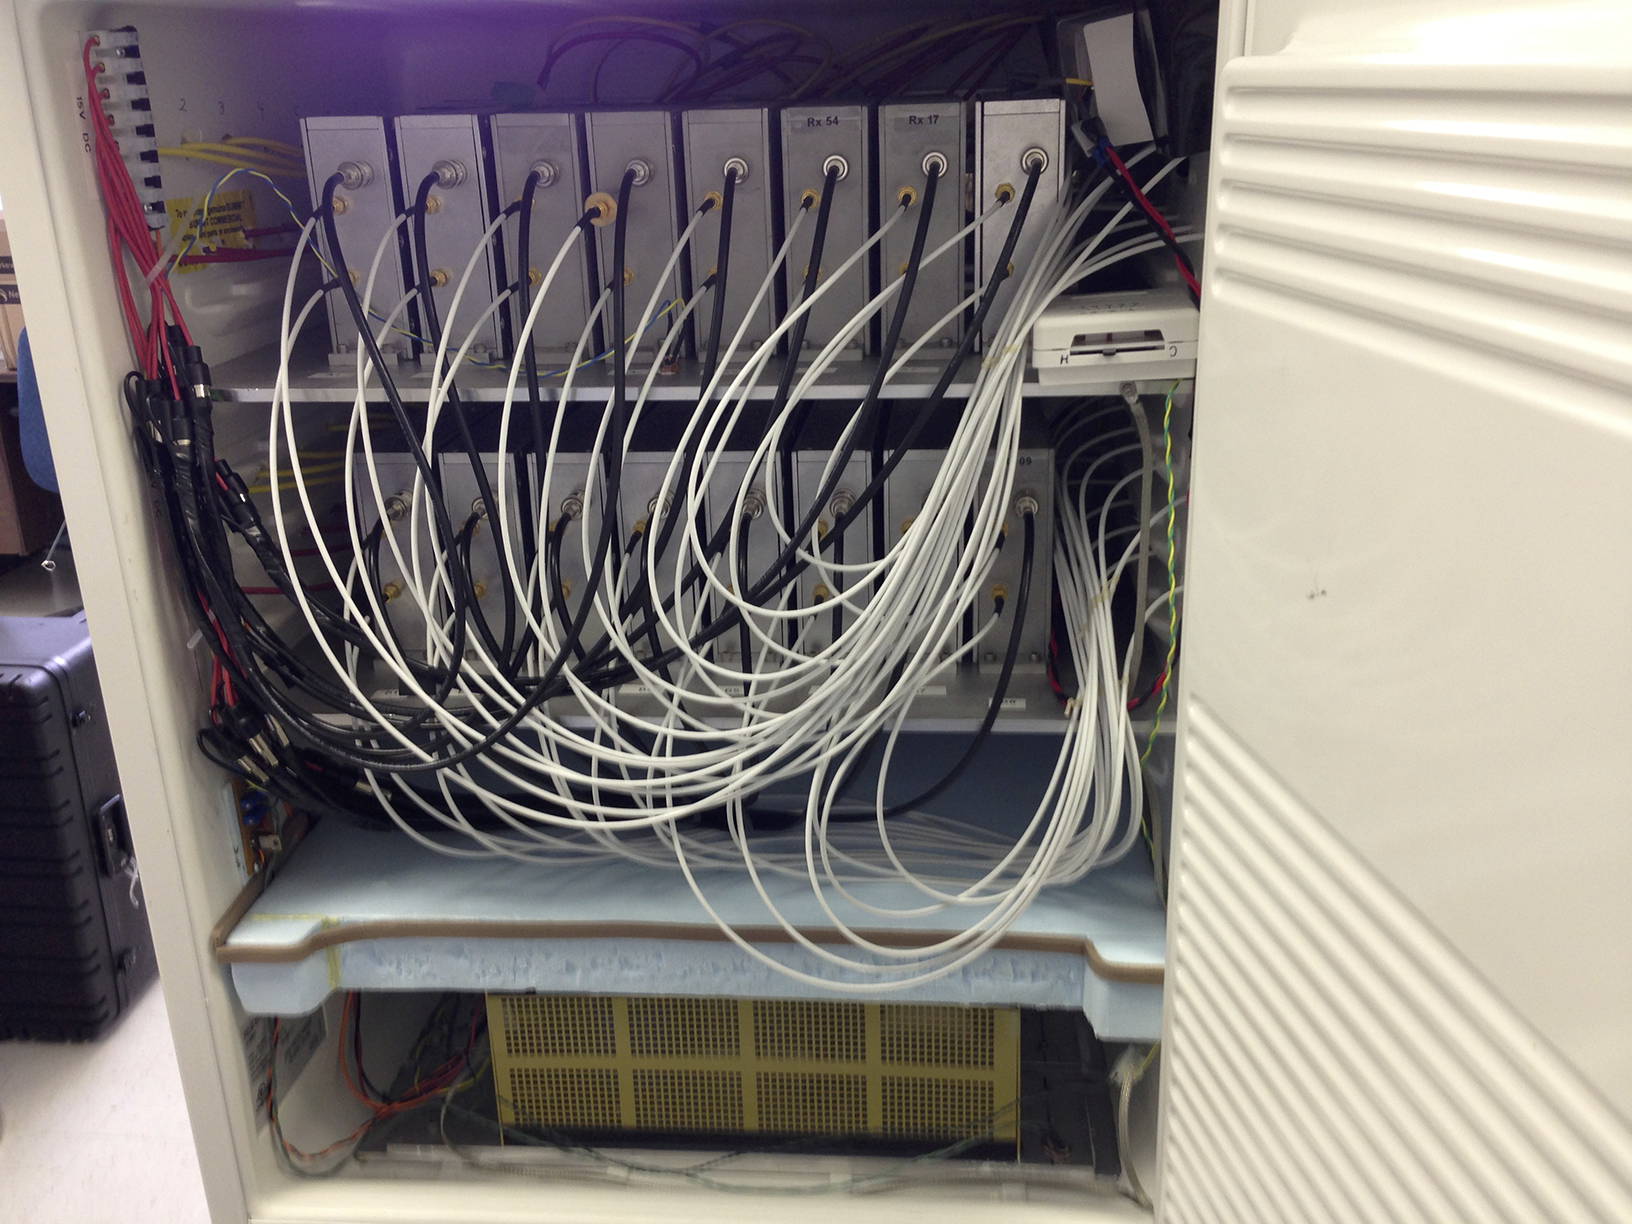
\includegraphics[width=2.7cm]{plots/recv_node.png}
        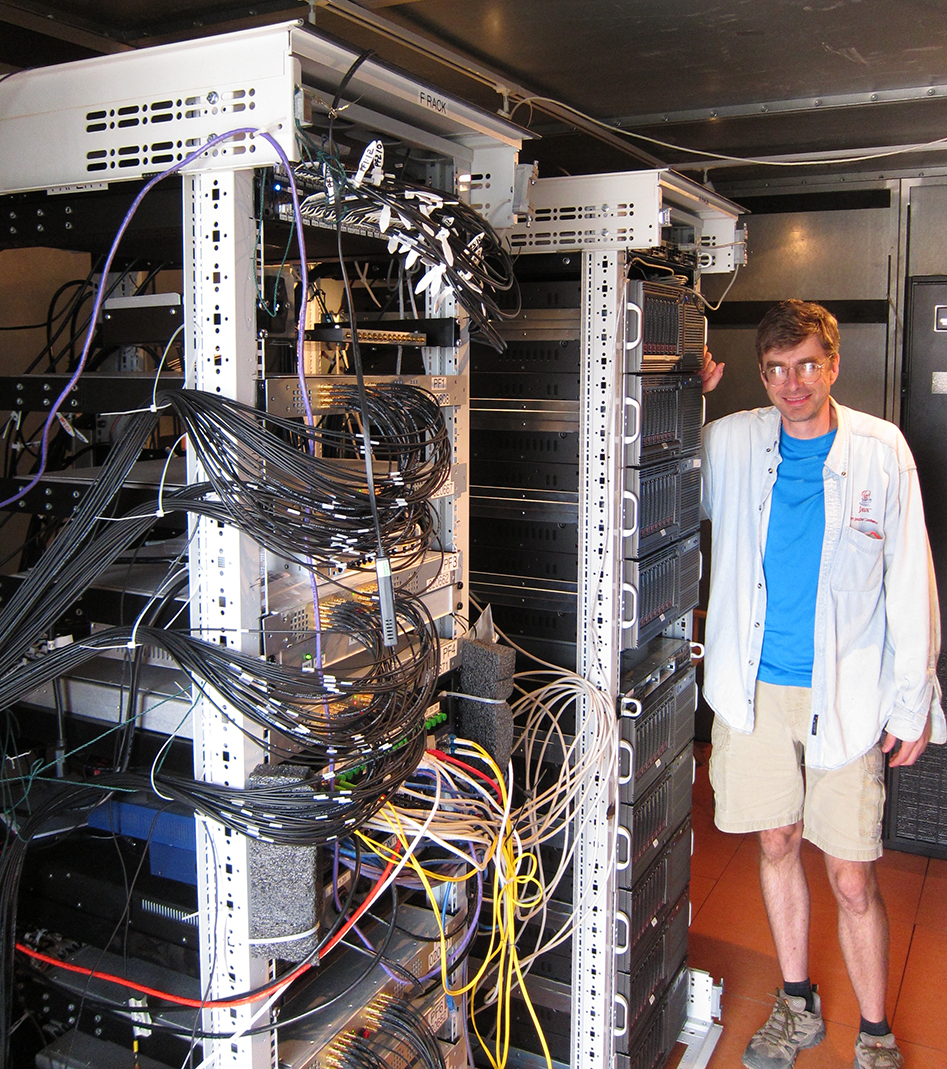
\includegraphics[width=2.7cm]{plots/digital.png}
    \caption{\small
    Existing components re-used in the HERA design include:
    the PAPER dipole antenna (left), 
    receivers in a node module (center), and
    the 128-element correlator deployed in the Karoo (right).}
\label{fig:components}
\end{figure}

%% TWO-COLUMN FIGURES

%f
\begin{figure*}[t]
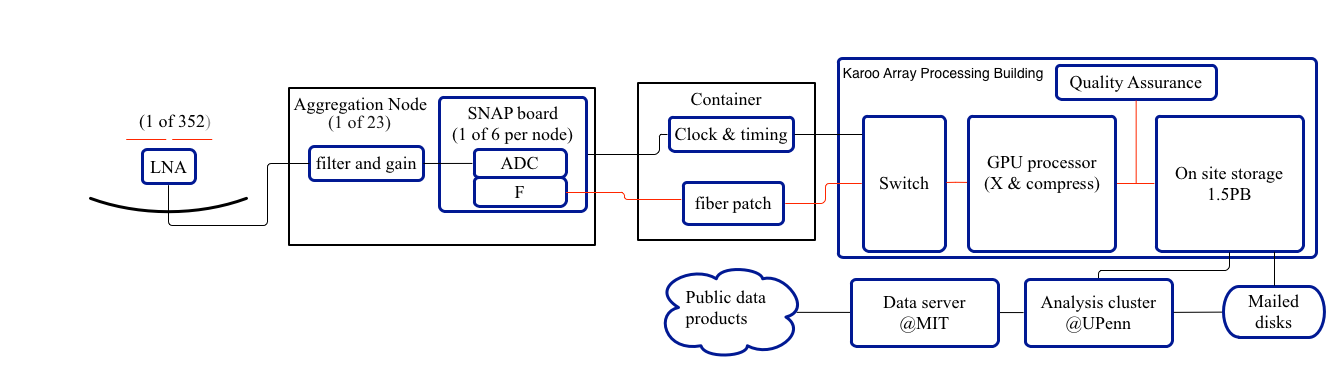
\includegraphics[width=12cm]{plots/HERA_high_level_block_diagram.png}
\caption{System}
\label{fig:systemOverview}
\end{figure*}

\begin{figure*}[t]
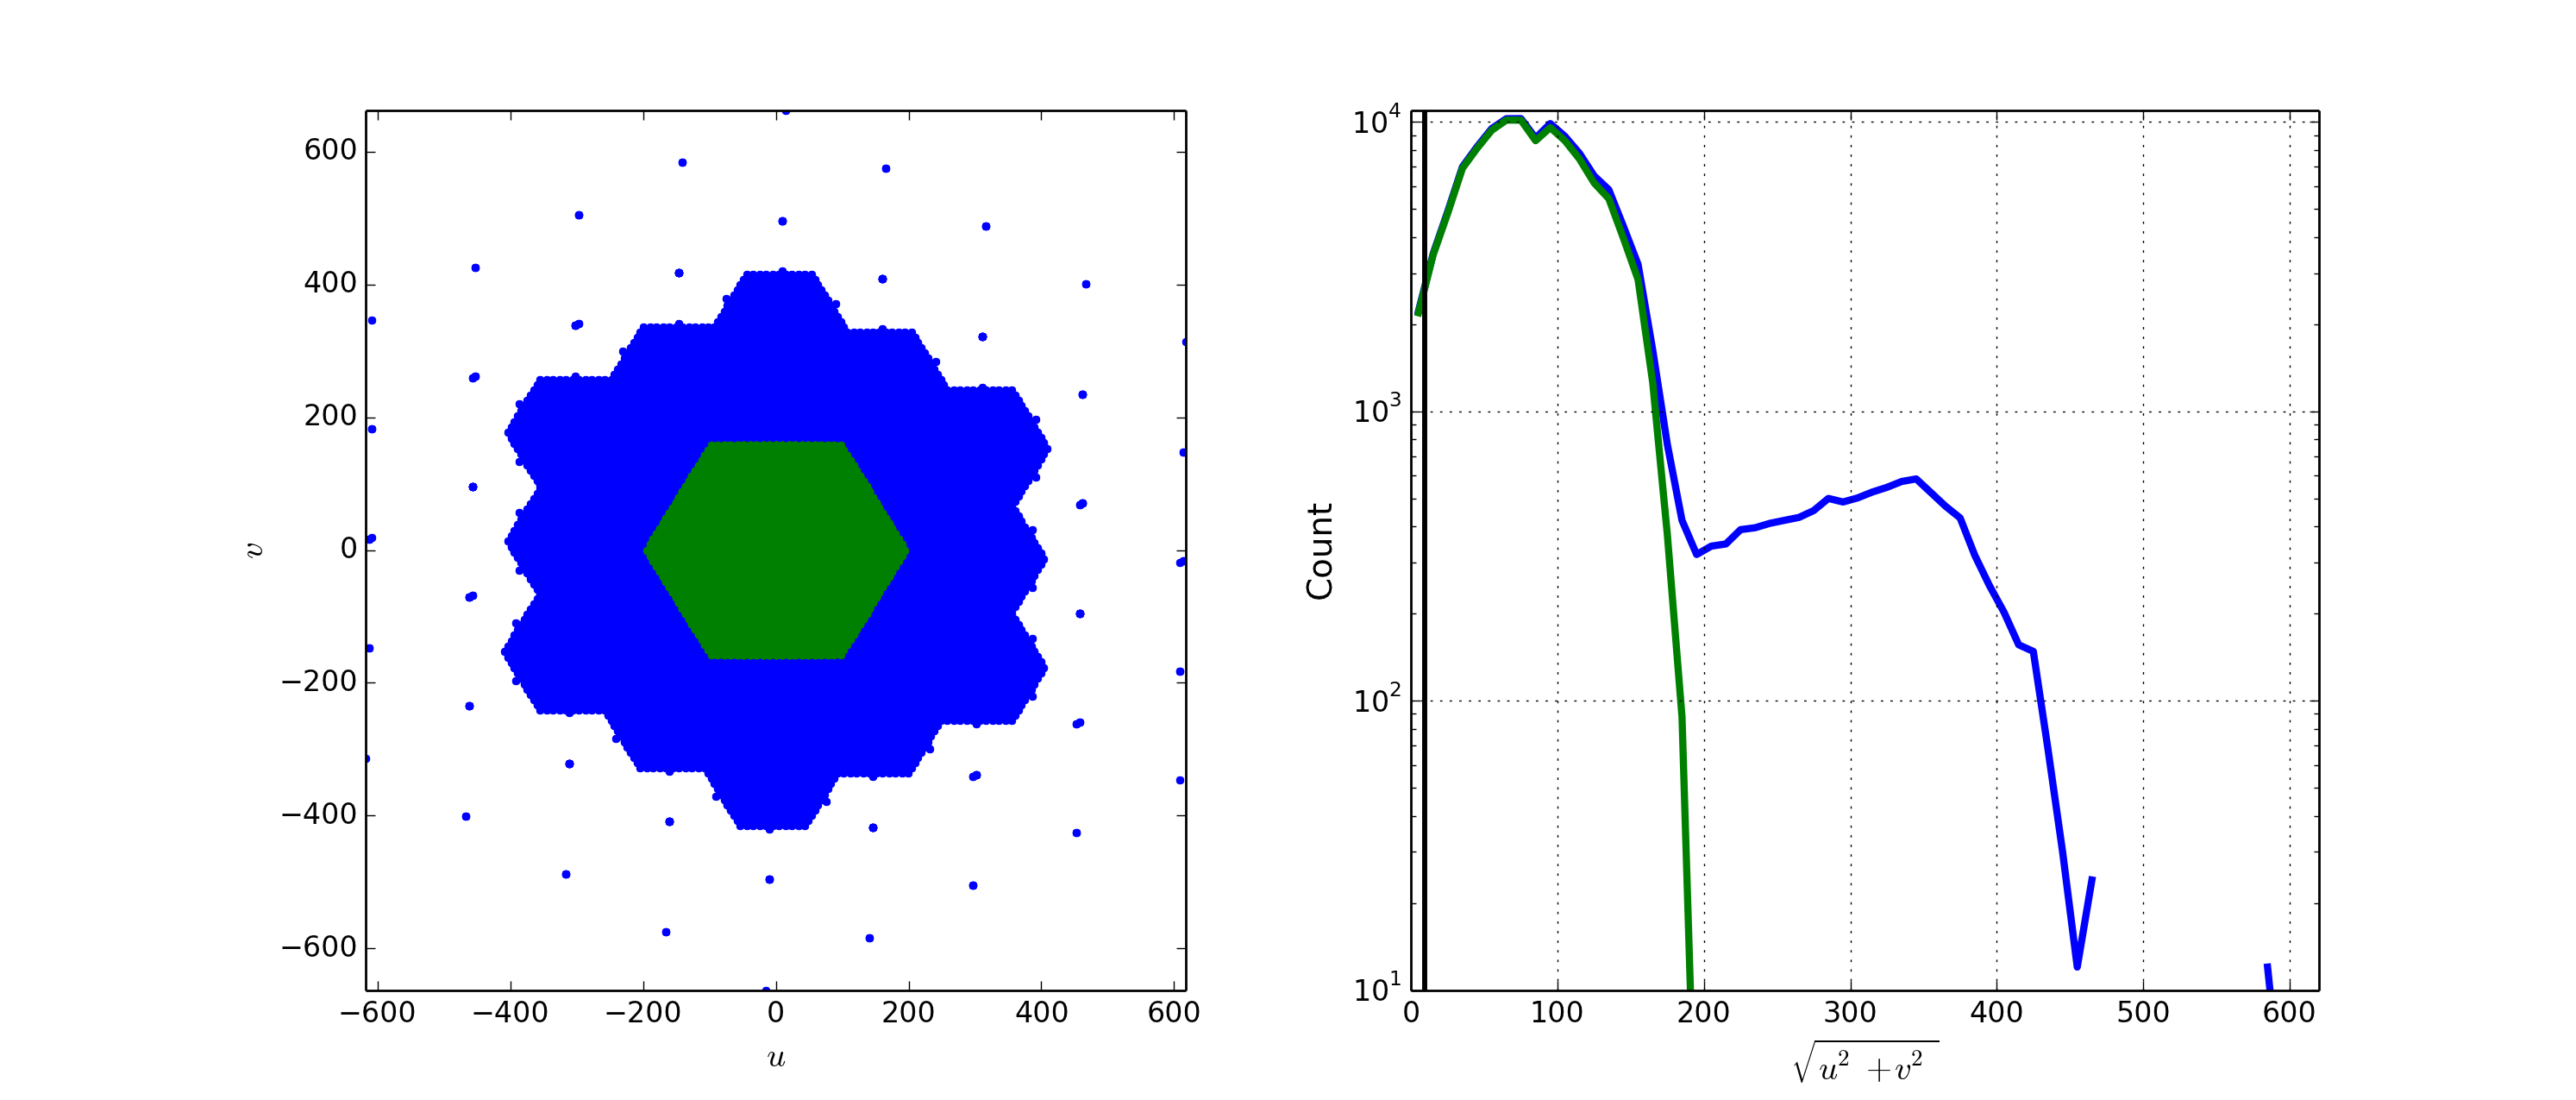
\includegraphics[width=12cm]{plots/config.png}
\caption{Configuration}
\label{fig:config}
\end{figure*}

%%%%%%%%%%%%%%%%%%%%%%%%%%%%%%%%%%%%%%%%%%%%%%%%%%%%%%%%%%%%%%%%%%%%
\begin{table*}[t]
\caption{HERA band in frequency, redshift, cosmic age and comoving distance.}
\label{tab:heraband}
\vskip4mm
\centering
\begin{tabular}{| c | c | c | c |} \hline
\textbf{Frequency [MHz]} & \textbf{Redshift} & \textbf{Age} & \textbf{Look-back} \\
\textbf{[MHz]}                   &                            & \textbf{[Myr]}  & \textbf{[Gly]} \\ \hline
50 & 27.4    & 164 & 13.6 \\ \hline
100 & 13.2  & 372 & 13.4 \\ \hline
200  & 6.1    & 960  & 12.8 \\ \hline
225  &  5.3   & 1,135  &  12.7 \\ \hline
\end{tabular}
\end{table*}

\begin{table*}[t]
\small
 \centering
 \begin{tabular}{c||r||r|r} 
%\begin{deluxetable}{c||r||r|r}
%\tabletypesize{\small}
%\tablecaption{\small
\hline
%\startdata
Instrument & Collecting Area (m$^2$) & Foreground avoidance & Foreground modeling \\
\hline
PAPER & 528 & 1.93 & 8.86 \\
MWA & 896 & 2.46 & 6.40 \\
LOFAR NL Core & 35,762 & 2.76 & 17.37 \\
\textbf{HERA-127} & \textbf{19,500} & \textbf{10.88} & \textbf{35.65} \\
\textbf{HERA-331} & \textbf{50,900} & \textbf{25.44} & \textbf{87.20} \\
SKA1 Low Core & 833,190 & 97.92 & 284.85 \\
%\enddata
\end{tabular}
\caption{Power spectrum signal-to-noise (``number of sigmas") at $z=9.5$ for various instruments, adapted from \citet{pober_et_al2014}.  By leveraging a filled, redundant configuration of dishes with high collecting area, HERA-331 allows high-significance power spectrum measurements using current foreground avoidance techniques, with further enhancements possible with likely advances in foreground modeling.}
\label{tab:signif}
\end{table*}

\begin{table*}[t]
\begin{tabular}{l | c | c} \hline
Parameter & Design & Performance\\  \hline
    Element diameter / FoV & 14 m & 9\arcdeg \\ 
    %Total collecting area & 54186 m$^2$ \\
    Min baseline length / largest scale & 14.6 m & 7.8\arcdeg \\
    Max core baseline length / synthesized beam & 306.6 m & 24\arcmin \\ 
    Max outrigger baseline length  & 1066.5 m & 9\arcmin \\
    Frequency / redshift range  & 50 - 250 MHz digitized \\
    & 70 - 230 MHz useable & 19.2 - 5.2 \\ 
    & 100 MHz correlated & \\
    Spectral channel width & 97.7 kHz & \\    
    System temperature / sensitivity & $100 + 120 (\nu/\rm{150~MHz})^{-2.55}$ K 
    & 50 $\mu \rm{Jy}~\rm{beam}^{-1}~\sqrt{\rm{hour}}$ \\
    \hline
%     At 150 MHz ($z=8.5$): & \\
%     ~{   }Naturally weighted synthesized beam FWHM & $24\arcmin$ \\
%     ~{   }Uniformly weighted synthesized beam FWHM & $9\arcmin$ \\
%     ~{   }Field of view FWHM & 9\arcdeg \\
%     ~{   }Point source RMS & 50 $\mu$Jy in 100 hrs \\
\end{tabular}
\caption{HERA-331 basic parameters.  Design parameters are connected to the derived instrument performance at 150 MHz.}
\label{tab:BasicParameters}
\end{table*}


%%%%%%%%%%%%%%%%%%%%%%%%%%%%%%%%%%%%%%%%%%%%%%%%%%%%%%%%%%%%%%%%%%%%
%% TABLES
%%
%% The different columns must be seperated with a & command and should
%% end with \\ to identify the column brake.

%% ONE-COLUMN TABLE

%t
%\begin{table}[t]
%\caption{TEXT}
%\begin{tabular}{column = lcr}
%\tophline
%
%\middlehline
%
%\bottomhline
%\end{tabular}
%\belowtable{} % Table Footnotes
%\end{table}


%% NUMBERING OF FIGURES AND TABLES
%%
%% If figures and tables must be numbered 1a, 1b, etc. the following command
%% should be inserted before the begin{} command.
%\addtocounter{figure}{-1}\renewcommand{\thefigure}{\arabic{figure}a}


%% MATHEMATICAL EXPRESSIONS

%% All papers typeset by Copernicus Publications follow the math typesetting regulations
%% given by the IUPAC Green Book (IUPAC: Quantities, Units and Symbols in Physical Chemistry,
%% 2nd Edn., Blackwell Science, available at: http://old.iupac.org/publications/books/gbook/green_book_2ed.pdf, 1993).
%%
%% Physical quantities/variables are typeset in italic font (t for time, T for Temperature)
%% Indices which are not defined are typeset in italic font (x, y, z, a, b, c)
%% Items/objects which are defined are typeset in roman font (Car A, Car B)
%% Descriptions/specifications which are defined by itself are typeset in roman font (abs, rel, ref, tot, net, ice)
%% Abbreviations from 2 letters are typeset in roman font (RH, LAI)
%% Vectors are identified in bold italic font using \vec{x}
%% Matrices are identified in bold roman font
%% Multiplication signs are typeset using the LaTeX commands \times (for vector products, grids, and exponential notations) or \cdot
%% The character * should not be applied as mutliplication sign

\end{document}
